\documentclass[11pt]{article}

% Required packages
\usepackage[margin=1in]{geometry}  % Page margins
\usepackage{setspace}              % For line spacing
\usepackage{times}                 % Times New Roman font
\usepackage{titlesec}              % For title formatting
\usepackage{fancyhdr}              % For page numbering
\usepackage{graphicx}              % For images
\usepackage{hyperref}              % For hyperlinks
\usepackage{amsmath}               % For math
\usepackage{booktabs}              % For tables
\usepackage{xcolor}                % For colors
\usepackage{float}                 % For figure positioning
\usepackage{caption}               % For caption formatting
\usepackage{kotex}                 % For Korean language support
\usepackage{algorithm}
\usepackage{algpseudocode}
% Set line spacing to double for main text
\doublespacing
\usepackage{enumitem}
\setlist[itemize]{leftmargin=0pt}

% Set single spacing for footnotes
\setlength{\footnotesep}{\baselineskip}
\renewcommand{\footnoterule}{%
  \kern -3pt
  \hrule width 2in height 0.4pt
  \kern 2.6pt
}

% Format section titles
\titleformat{\section}{\normalfont\fontsize{16pt}{19pt}\bfseries}{\thesection}{1em}{}
\titleformat{\subsection}{\normalfont\fontsize{14pt}{17pt}\bfseries}{\thesubsection}{1em}{}

% Page numbering
\pagestyle{fancy}
\fancyhf{}
\renewcommand{\headrulewidth}{0pt}
\cfoot{\thepage}

% Citation style - use square brackets
\makeatletter
\renewcommand\@biblabel[1]{[#1]}
\makeatother

% Figure and table caption formatting
\captionsetup[figure]{position=bottom, justification=centering, font=normal}
\captionsetup[table]{position=top, justification=centering, font=normal}

\begin{document}

%-------------------------------------------------------------------------------
% 외표지 (Cover Page)
%-------------------------------------------------------------------------------
\begin{titlepage}
\begin{center}
\vspace*{1cm}
{\fontsize{21pt}{25pt}\selectfont\bfseries Integrating Vision Language Model based Rewards
with World Foundation Model based Reinforcement Learning\par}
\vspace{0.5cm}
{\fontsize{16pt}{19pt}\selectfont\bfseries (비전-언어 모델 기반 보상과 모델 기반 강화학습의 통합)\par}
\vspace{5cm}
{\fontsize{16pt}{19pt}\selectfont 2025년 5월 \par}
\vspace{3cm}
{\fontsize{16pt}{19pt}\selectfont 서울대학교 공과대학\par}
{\fontsize{16pt}{19pt}\selectfont 전기·정보공학부\par}
{\fontsize{16pt}{19pt}\selectfont 박 경 서\par}
\vspace{1.5cm}

\end{center}
\end{titlepage}

%-------------------------------------------------------------------------------
% 인준지 (Approval Page)
%-------------------------------------------------------------------------------

%-------------------------------------------------------------------------------
% 영문초록 (English Abstract) - 영문 논문이므로 영문초록이 먼저 나옴
%-------------------------------------------------------------------------------
\pagenumbering{roman} % 로마자 소문자로 페이지 번호 시작

\begin{center}
\Large\textbf{Abstract}
\end{center}
\vspace{1cm}

This paper proposes LIVerse( \textbf{L}anguage \& \textbf{I}mage integrated uni\textbf{Verse} model), a novel world foundation model (WFM) that unifies vision-language semantics and forward dynamics into a unified latent space to enhance the generality and scalability of model-based reinforcement learning. Unlike traditional imitation learning-based robot foundation models (RFMs), we introduce a PlaNet-style agent that leverages vision-language model (VLM) based reward in sampling-based model predictive control (MPC) manner. To overcome the limitations of cosine similarity rewards in complex tasks, we adopt step-wise planning and propose a delta-score reward function that measures incremental similarity improvements, thereby addressing the reward scale mismatch problem across sub-tasks. Through extensive experiments on the Meta-World benchmark, LIVerse based MPC agent demonstrates strong zero-shot policy execution, transfer learning across diverse tasks, and effective sub-task decomposition. It significantly reduces the dependency on hand-crafted rewards and enables zero-shot reward models to be extended into zero-shot policy models. As a result, this work presents a new paradigm for RFM that integrate model-based reinforcement learning with LIVerse.

\vspace{1cm}
\noindent\textbf{Keywords}: Vision-Language Model based Reward, Model-Based Reinforcement Learning, Model Predictive Control, World Foundation Model, Robot Foundation Model\\
\vspace{0.5cm}
\noindent\textbf{Student Number}: 2020-12295

\clearpage

%-------------------------------------------------------------------------------
% 목차 (Table of Contents)
%-------------------------------------------------------------------------------
\tableofcontents
\clearpage
\listoffigures
\clearpage

%-------------------------------------------------------------------------------
% 본문 (Main Content)
%-------------------------------------------------------------------------------
%%%%%%%%%%%%%%%%%%%%%%%%%%%%%%%%%%%%%%%%%%%%%%%%%%%%%%%%%%%%%%%%%%%%%%%%%%
%%%%%%%%%%%%%%%%%%%%%%%%%%%%%%%%%%%%%%%%%%%%%%%%%%%%%%%%%%%%%%%%%%%%%%%%%%
\pagenumbering{arabic} % 아라비아 숫자로 페이지 번호 시작

\section{Introduction}

\subsection{Goal of the paper}
\begin{itemize}
    \item \textbf{Understanding Vision Language Model based Reward Model in Reinforcement Learning}: This paper aims to explore and analyze how Vision Language Models (VLMs) can serve as Reward Models (RMs) in reinforcement learning (RL), providing a framework for robots to understand and execute general tasks described in natural language and visual observations.
    
    \item \textbf{Integrating VLM-RM with World Foundation Model}: We investigate the potential of combining VLM-RM with learned world models to enhance task generalization in robotic control tasks. We propose \textit{\textbf{LIVerse}}, a World Foundation Model (WFM) that understands both forward dynamics of agent system and semantics of visuo-linguistic information  in a unified latent space.

    \item \textbf{Proposing new approach to Robot Foundation Models}: We introduce a novel approach to Robot Foundation Models (RFMs) that departs from imitation learning based methods and embraces model-based planning with a WFM. By incorporating sampling-based MPC on top of learned WFM, our approach leverages VLMs as zero-shot reward models rather than directly as action modules, enabling more flexible and generalizable robotic systems.
\end{itemize}

\subsection{Vision Language Model}
\begin{itemize}
    \item \textbf{Various VLMs}: VLMs are foundation models trained to understand and process both visual and textual information. In this work, we consider encoder-based vision-language multimodal models like CLIP \cite{clip}, ALIGN, and Florence that can associate images with text descriptions, enabling cross-modal understanding and reasoning. 
    
    \item \textbf{Image and Text Encoder}: The fundamental architecture of VLMs typically includes an image encoder (often a convolutional neural network or vision transformer) and a text encoder (typically a transformer-based language model). These encoders map images and text into a shared embedding space. The embedding space captures the semantic meaning of both visual and textual modalities.
    
    \item \textbf{Objective functions}: VLMs are commonly trained using contrastive learning objectives, where the model learns to maximize the similarity between embeddings of matched image-text pairs while minimizing similarity between unmatched pairs. Other objectives include masked language modeling and image-text matching.
    
    
\end{itemize}

\subsection{Reward of Reinforcement Learning}
\begin{itemize}
    \item \textbf{Basic RL problem}: Reinforcement learning is formulated as a Markov Decision Process (MDP) where an agent learns to maximize cumulative rewards by interacting with an environment. The fundamental components include states, actions, transition dynamics, rewards, and a discount factor.
    
    \item \textbf{Reward and Task}: In RL, tasks are defined implicitly through reward functions. For example, in locomotion tasks for quadrupedal robots, rewards typically combine terms for tracking command velocity, energy efficiency, stability metrics, penalty terms for undesirable configurations and behaviors, etc. The total reward function can be decomposed as:
    
    \begin{equation}
    R_{total} = w_v R_{velocity} + w_e R_{energy} + w_s R_{stability} + w_p R_{penalty}
    \end{equation}
    
    where $w_v$, $w_e$, $w_s$, and $w_p$ are weighting coefficients for each reward component.
    
    \textbf{Velocity Tracking Reward}: Encourages the robot to follow desired velocity commands:
    \begin{equation}
    R_{velocity} = \exp\left(-\frac{||\mathbf{v}_{cmd} - \mathbf{v}_{actual}||^2}{\sigma_v^2}\right)
    \end{equation}
    where $\mathbf{v}_{cmd}$ is the commanded velocity, $\mathbf{v}_{actual}$ is the actual velocity, and $\sigma_v$ controls the sensitivity.
    
    \textbf{Energy Efficiency Reward}: Penalizes excessive energy consumption:
    \begin{equation}
    R_{energy} = -\sum_{i=1}^{n_{joints}} |\tau_i \cdot \dot{q}_i|
    \end{equation}
    where $\tau_i$ and $\dot{q}_i$ are the torque and angular velocity of the $i$-th joint respectively.
    
    \textbf{Stability Reward}: Promotes stable locomotion by rewarding proper body orientation:
    \begin{equation}
    R_{stability} = \exp\left(-\frac{||\mathbf{q}_{base} - \mathbf{q}_{desired}||^2}{\sigma_s^2}\right) - \beta ||\boldsymbol{\omega}_{base}||^2
    \end{equation}
    where $\mathbf{q}_{base}$ is the base orientation quaternion, $\mathbf{q}_{desired}$ is the desired orientation, $\boldsymbol{\omega}_{base}$ is the base angular velocity, and $\beta$ is a damping coefficient.
    
    \textbf{Penalty Terms}: Discourage undesirable behaviors such as joint limit violations and foot slippage:
    \begin{equation}
    R_{penalty} = -\lambda_1 \sum_{i=1}^{n_{joints}} \mathbb{I}(q_i \notin [q_{i,min}, q_{i,max}]) - \lambda_2 \sum_{j=1}^{n_{feet}} ||\mathbf{v}_{slip,j}||
    \end{equation}
    where $\mathbb{I}(\cdot)$ is the indicator function, $q_{i,min}$ and $q_{i,max}$ are joint limits, $\mathbf{v}_{slip,j}$ is the slip velocity of the $j$-th foot, and $\lambda_1$, $\lambda_2$ are penalty weights.
    
    
    \item \textbf{Design of reward function}: Like the example above, designing reward functions for every task through a combination of complex scalar functions is a difficult task and has poor scalability. But traditional RL relies on manually designed reward functions, which becomes increasingly challenging for complex tasks. Crafting effective reward functions requires domain expertise and extensive tuning. Many real-world tasks are difficult to express as a scalar function, particularly when objectives are ambiguous and fuzzy. Can we design a reward function for the task of "Sit next to me and help me do laundry"?
\end{itemize}

\subsection{Vision Language Model as Reward Model}
\begin{itemize}
    \item \textbf{CLIP based Cosine-Similarity}: CLIP-based reward models are the most basic reward form that leverages the shared embedding space of vision and language to compute rewards. By calculating the cosine similarity between the embedding of the current visual observation and the embedding of the target text description, these models provide a measure of task achievement.
    
    \item \textbf{Preference Learning}: Some approaches use VLMs to provide preference signals between different behaviors or states. These preferences can then inform reward learning processes or direct policy optimization without explicitly constructing a reward function.
    
    \item \textbf{Code Generator}: Advanced ChatGPT-style VLMs can generate code for reward functions based on task descriptions and observations. This method, exemplified by Eureka \cite{eureka}, generates rewards well for tasks frequently used in RL.
\end{itemize}

However, preference learning and code generation approaches face limitations in terms of generalization and scalability. Therefore, in this work, we adopt the most fundamental form of VLM RM : CLIP-style Cosine-Similarity reward.

\subsection{Model based Reinforcement Learning}
\begin{itemize}
    \item \textbf{Learning World Model}: Model-based Reinforcement Learning (MBRL) involves learning a model of the environment's dynamics through real world interactions. This world model typically includes forward dynamics prediction and may incorporate reward prediction, state reconstruction, and other predictive components.
    
    \item \textbf{Dreamer-style MBRL}: Approaches like Dreamer \cite{dreamer} leverage world models to enhance sample efficiency by imaginary rollouts. They enable actor-critic methods to learn from these simulated experiences. This significantly improves sample efficiency as the agent can learn from imagined trajectories without additional environment interactions.
    
    \item \textbf{PlaNet-style MBRL}: Approaches like PlaNet \cite{planet} use world models with sampling-based Model Predictive Control (sampling-based MPC) methods like the Cross Entropy Method (CEM) or Model Predictive Path Integral (MPPI). These methods optimize action sequences by repeatedly simulating their trajectory using the world model and optimizing them to maximize expected rewards.
\end{itemize}

In this work, we propose MBRL that implements both style of MBRL, but utilizes PlaNet-style MPC as the main framework.

\subsection{Robot Foundation Model}
\begin{itemize}
    \item \textbf{Current Robot Foundation Models}: Most RFMs rely on Imitation Learning (IL) frameworks like Behavior Cloning, where policies are learned directly from expert demonstrations. RFMs combine language and vision foundation models to enable task generalization through text descriptions and observation generalization through image frames. Also, recent advances in RFM have evolved by combining generative models to policy like diffusion model, flow-mathcing model. As the RT-series \cite{rt1,rt2} begins, RFMs such as OpenVLA \cite{openvla}, PI0 \cite{pi0}, and GR00T-N1 \cite{gr00t} are being developed.

    
    \item \textbf{Limitations of Robot Foundation Models}: Current RFMs lack of explicit control/planning components. As a result, they lack the ability to perform goal-directed behavior under varying task objectives and physical constraints in long-horizon manner. In addition, generative policies have the inherent limitation of making it difficult to maintain temporal consistency. They not only produce suboptimal solutions due to the lack of optimization and prediction capabilities, but also suffer from unpredictability as a drawback. Without an integrated notion of system dynamics, physical constraints, feedback loop, hierarchical planning schemes, RFMs are fundamentally limited to scalability for an actual robot system.
For example, there exists a disconnection between RL-driven locomotion research and IL-driven manipulation research, limiting the development of unified approaches.
Furthermore, the scalability of current RFMs is further hindered by the scarcity of large-scale expert demonstration datasets, which are essential for imitation learning. Collecting high-quality demonstrations across diverse robotic platforms, environments, and tasks is both labor-intensive and domain-specific, leading to poor generalization and transferability. This data bottleneck becomes even more pronounced in multi-embodiment settings, where heterogeneous morphologies demand different control strategies. Compounding this issue is the absence of standardized representations for actions and states across different robot embodiments, making it difficult to align experiences and knowledge across domains. Without a shared latent structure that unifies semantic, spatial, and temporal information across diverse agents, current RFMs cannot effectively benefit from shared learning or cross-domain transfer. 
These challenges emphasize the need for a new paradigm that goes beyond imitation and incorporates model-based planning, and world model-driven generalization.

\end{itemize}

\subsection{Contributions}
\textit{We propose \textbf{LIVerse}, a novel World Foundation Model that unifies the agent's physical dynamics with vision-language semantics in a shared latent space. \\
We propose \textbf{sampling-based MPC framework} that operates directly on top of the LIVerse, as a \textbf{zero-shot policy}. \\
We propose \textbf{delta score-based reward function} that enables \textbf{step-wise planning} to overcome the limitations of CLIP-style reward signals.\\}
Our integrated approach bridges the gap between model-based reinforcement learning and robot foundation models, enabling more generalizable and scalable to real robotic systems.

\section{VLM based Reward Model}

\subsection{CLIP}
\begin{itemize}
    \item \textbf{Key features}: CLIP is a pioneering vision-language model trained on 400 million image-text pairs using a contrastive learning objective. It maps images and texts into a shared embedding space, enabling zero-shot classification and cross-modal retrieval.
    
    \item \textbf{Limitations}: CLIP lacks temporal modeling capabilities and cannot track task progression over time. We can use cosine similarity score as rewards, but the static representations of CLIP limit adaptability in sequential decision making.
\end{itemize}

\subsection{R3M}
\begin{itemize}
    \item \textbf{Key features}: R3M \cite{r3m} learns a reusable visual representation from large-scale human egocentric videos using time-contrastive learning and video-language alignment. It captures both temporal and semantic structures and significantly boosts data efficiency when used as a frozen encoder in downstream manipulation tasks.
    
    \item \textbf{Limitations}: While, R3M ensures temporlal awareness, it does not provide explicit reward signals. It is not designed for planning or reinforcement learning, and lacks mechanisms for dynamic goal adaptation or optimization-based policy synthesis.
\end{itemize}

\subsection{Voltron}
\begin{itemize}
    \item \textbf{Key features}: Voltron \cite{voltron} introduces a language-driven visual representation learning framework that combines masked autoencoding with language conditioning and generation. It learns both low-level spatial patterns and high-level semantics and demonstrates robust transfer across a wide spectrum of robot learning tasks.
    
    \item \textbf{Limitations}: Voltron is not designed as a reward model and lacks mechanisms for computing goal-conditioned rewards. While it excels in semantic understanding, it does not explicitly support reward shaping, planning, or policy optimization.
\end{itemize}

\subsection{VIP}
\begin{itemize}
    \item \textbf{Key features}: VIP \cite{vip} proposes a self-supervised value-implicit pretraining method that treats human video data as an offline goal-conditioned RL problem. It learns temporally smooth embeddings where distances between current and goal frames provide dense reward signals without requiring actions or annotations.
    
    \item \textbf{Limitations}: VIP is limited to image-based goal specification and cannot process language commands. It lacks integrated semantic understanding and hierarchical reward decomposition, and its value function is not directly connected to explicit planning or control modules.
\end{itemize}

\subsection{LIV}
\begin{itemize}
    \item \textbf{Key features}: LIV \cite{liv} extends VIP by integrating language inputs into the value-learning framework, enabling dense reward computation from either image or language goals. It unifies VIP and CLIP principles to jointly learn multimodal representations and value functions from video-language data.
    
    \item \textbf{Limitations}: LIV still struggle with long or ambiguous natural language instructions. Even though LIV incorporate temporal relations and semantic rounding through language, their actual performace as reward models remains insufficient for practical RL applications.
\end{itemize}

In this work, we adopt a LIV-based reward model due to its key advantages: it provides dense, language-conditioned rewards by jointly learning visual and linguistic representations.

\subsection{Overall Limitations of CLIP-style Reward Models}
\begin{itemize}
    \item \textbf{Limitations of Vision-Language Models (VLMs)}: Pretrained VLMs, such as CLIP, often produce \emph{fuzzy and imprecise reward signals} due to their limited lingual, spatial understanding, lack of temporal understanding, and dependence on training data distribution. These models may struggle with tasks involving dynamic interactions or fine-grained spatial relations, and their generalization ability is sensitive to domain shift. Furthermore, the quality of reward output is strongly correlated with the scale and training diversity of the VLM, making lightweight or out-of-domain deployments less reliable. In practice, agents trained with such fuzzy reward signals are prone to getting stuck in \emph{local optima}, as the rewards may not accurately reflect true task progression.
    
    \item \textbf{Limitations of Cosine Similarity-based Reward Functions}: CLIP-style reward models use cosine similarity between the image observation and a text description. By introducing a simple dynamics system and constraints of the norm of embedding vector, we can derive a policy that maximizes the objective, which always takes as big steps as possible to the goal state.
This induces agent to move directly toward a target embedding in latent space. However, in real-world robotics tasks with physical and temporal constraints, this leads to suboptimal behavior. The optimal trajectory in the embedding space does not map to the otimal trajectory in the task space. As the trajectory non-linearity increases, the semantic distance in the embedding space may poorly correlate with task success, making such reward structures ineffective for long-horizon planning or hierarchical task decomposition.
\[
\begin{aligned}
\textbf{Reward:} \quad & r(x) = \frac{x^\top x^*}{\|x\| \, \|x^*\|} \quad \\
\textbf{Dynamics:} \quad & x_{t+1} = \frac{x_t + a}{\|x_t + a\|} \quad \left( \|x_t\| = 1 \right) \\[1.5ex]
\textbf{Optimal Policy:} \quad & \pi^*(x) = \lambda(x^* - x)
\end{aligned}
\]
\end{itemize}

These limitations highlight the need for improved reward modeling approaches that combine the semantic generalization of VLMs with the structure and feedback of model-based planning or learned reward shaping.


\section{VLM RM based RL}

\subsection{VLM-RMs}
\begin{itemize}
    \item \textbf{Key features}: VLM-RMs \cite{vlmrm} uses CLIP to provide reward signals from simple language prompts like “a humanoid robot kneeling,” eliminating the need for hand-crafted reward functions for reinforcement learning. They compute rewards using the cosine similarity between an image observation and a natural language task description, enabling task specification via simple prompts. The method introduces goal-baseline regularization to improve discriminative power and robustness.

    \item \textbf{Limitations}: The effectiveness of VLM-RMs heavily depends on the VLM's pretraining quality and capacity. They can suffer from misalignment in visually ambiguous environments or lack spatial reasoning. Also, the reward signal may not reflect fine-grained temporal task progress, limiting performance in long-horizon or multi-stage tasks.
\end{itemize}

\subsection{RoboCLIP}
\begin{itemize}
    \item \textbf{Key features}: RoboCLIP \cite{roboclip} is an imitation learning framework that uses a single demonstration — either a video or a text description — to generate rewards using pretrained video-language models (S3D). It provides sparse trajectory-level reward signals and achieves zero-shot generalization.

    \item \textbf{Limitations}: RoboCLIP relies on episodic (trajectory-level) reward signals, which can hinder fine-grained temporal credit assignment. It assumes good alignment between pretrained VLM features and the robot’s task space, and may struggle in domains with visual-domain shift or fine control requirements.
\end{itemize}

\subsection{RL-VLM-F}
\begin{itemize}
    \item \textbf{Key features}: RL-VLM-F \cite{rlvlmf} learns reward model by pairwise preferences over image observations, obtained by querying VLMs based on task descriptions. This preference-based reward learning removes the need for ground-truth states or human feedback.

    \item \textbf{Limitations}: The method involves multiple rounds of querying VLMs, which can be computationally expensive. Preference-based training based on VLM querying has black-box interpretability.
\end{itemize}

\subsection{FuRL}
\begin{itemize}
    \item \textbf{Key features}: FuRL \cite{furl} addresses the “fuzzy reward” problem caused by VLM reward misalignment by introducing reward alignment via lightweight projection layers and relay RL for exploration. It fine-tunes VLM embeddings minimally to better reflect task progress and uses relay mechanisms to escape local optima, improving performance in sparse reward settings.

    \item \textbf{Limitations}: FuRL relies on the successful trajectory and task specific rewards, which reduces scalability. It introduces additional components to the training loop (alignment modules, relay agents), increasing system complexity.
\end{itemize}

\subsection{Overall Limitations of VLM-RM based RL}
\begin{itemize}
    \item \textbf{Auxiliary Role of VLM Rewards}: In most frameworks, VLM-based rewards serve only as auxiliary signals, acting as intrinsic rewards to complement hand-designed task rewards.

    \item \textbf{Task-Specific Optimization}: Techniques to improve the quality of VLM-derived rewards—such as fine-tuning for reward alignment or learning preference-based reward models—require task-specific supervision or pairwise feedback. These approaches inherently optimize for a \emph{single task}, and are not easily generalizable to multi tasks. As a result, such agents lack scalability to \emph{multi-task learning} or \emph{transfer learning} scenarios.
\end{itemize}

In conclusion, while all methods are training agents optimized for a single task, they face a fundamental limitation: each time the task, observation space, environment dynamics, or constraints change, the agent must be retrained from scratch.

\section{LIVerse: A World Foundation Model Unifying Dynamics and Semantics}

\subsection{Proposed World Foundation Model}
We propose \textbf{LIVerse} (\textbf{L}anguage \& \textbf{I}mage integrated uni\textbf{Verse} model) \autoref{fig:LIVerse}, a novel World Foundation Model. LIVerse combines a latent space based on Recurrent State Space Model (RSSM), which encodes the agent's latent dynamics, with a vision-language embedding space learned from LIV\cite{liv}, a pre-trained VLM encoder. This joint latent space supports both model-based planning and policy learning by serving as the learned world model for our MBRL agent.

LIVerse provides \textit{imaginary rollouts} in a model-predictive manner, which can be used for both generating trajectories in Actor-Critic training and trajectory optimization in MPC. While the model is \emph{embodiment-dependent}—which need to be trained for each robotic platform—it is \textbf{task-agnostic}, enabling generalization across various tasks. This allows the same world model to be reused for different tasks, supporting multi-task reinforcement learning and meta-reinforcement learning. Furthermore, when integrated with MPC, it constitutes a new form of RFM.

\begin{figure}
    \centering
    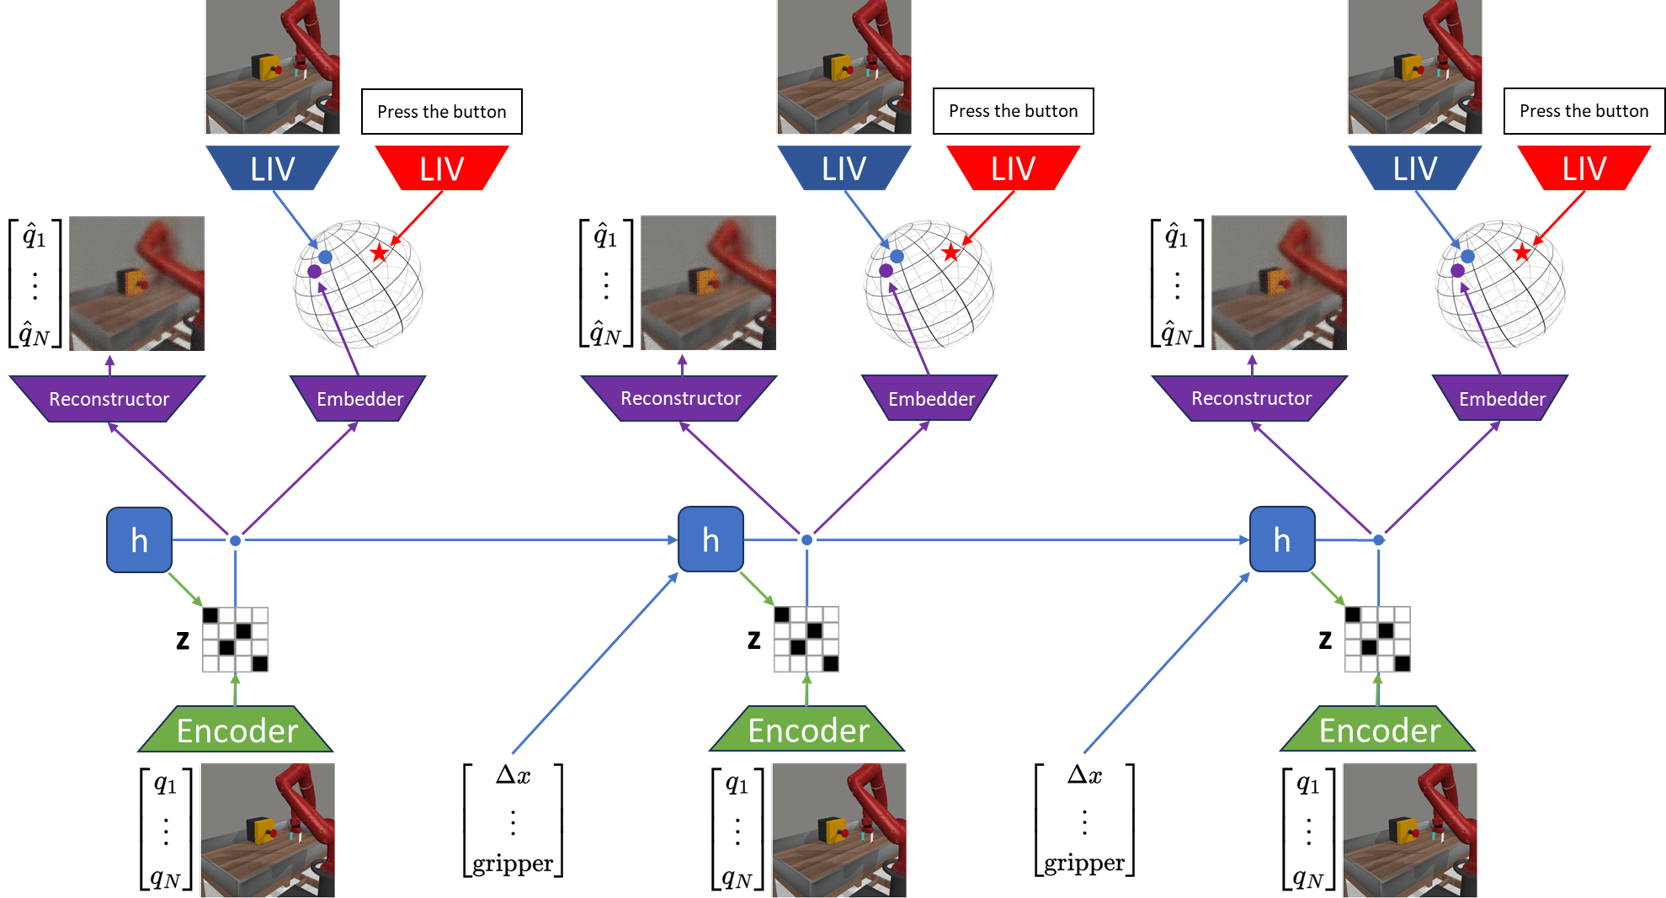
\includegraphics[width=1\linewidth]{LIVerse.png}
    \caption{LIVerse}
    \label{fig:LIVerse}
\end{figure}


\subsection{Dreamer based Implementation}
The model implementation follows the basic architecture of DreamerV3, and also utilizes detail components such as symlog transformation, free bits regularization, and straight-through gradients for categorical latents. These implementation details are not the primary focus of our contribution. For full technical reference, we refer the reader to \textit{Mastering Diverse Domains through World Models} (DreamerV3)\cite{dreamer}. Unlike the original DreamerV3 world model, which includes a reward predictor, LIVerse eliminates this component and instead introduces a Language-Image Embedder that predicts the semantic embedding vector of the current image in the shared language-image space.

\subsection{Components of LIVerse}
\textbf{1. Recurrent State Space Model (RSSM)}\\
RSSM captures the agent's latent forward dynamics via recurrent unit like GRU cells.
\begin{itemize}
\setlength\itemindent{20pt}
    \item \textbf{Encoder}: Encodes observations (image frame $I_t$ and robot state $q_t$) into stochastic latent variables $z_t$.
\begin{equation}
z_t \sim q_\phi(z_t \mid h_t, I_t, q_t)
\end{equation}
    \item \textbf{Recurrent Dynamics}: Predicts the next recurrent state $h_t$ from the previous recurrent state $h_{t-1}$, action $a_{t-1}$, and stochastic latent $z_{t-1}$.
\begin{equation}
h_t = f_\phi(h_{t-1}, z_{t-1}, a_{t-1})
\end{equation}
    \item \textbf{Transition Predictor}: Predicts the next stochastic latent $z_t$ using only $h_t$, i.e., without observing $I_t$ and $q_t$, modeling forward dynamics independently from observation.
\begin{equation}
\hat{z}_t \sim p_\phi(\hat{z}_t \mid h_t)
\end{equation}
\end{itemize}

\textbf{2. Prediction Heads}\\
Predict obeservations and VLM embedding vectors from the recurrent state $h_t$ and stochastic state $z_t$.
\begin{itemize}
\setlength\itemindent{20pt}
    \item \textbf{LIV Image Embedder}: Predicts the LIV image embedding $e_{I_t}$ corresponding to the current image frame. This replaces the traditional reward predictor in Dreamer models and decodes visuo-linguistic semantics. So instead of predicting environment rewards directly, the model learns to predict embeddings that maximize cosine similarity with the real LIV image embedding.
\begin{equation}
\hat{e_I}_t \sim p_\phi(\hat{e_I}_t \mid h_t, z_t)
\end{equation}
    \item \textbf{Image Frame Reconstructor}: Reconstructs the image frame $I_t$. While not directly used during inference, it supports training of the LIV image embedder by regularizing visual feature learning.
\begin{equation}
\hat{I}_t \sim p_\phi(\hat{I}_t \mid h_t, z_t)
\end{equation}
    \item \textbf{Robot State Reconstructor}: Reconstructs robot state $q_t$ to help the model learn accurate physical dynamics during training.
\end{itemize}
\begin{equation}
\hat{q}_t \sim p_\phi(\hat{q}_t \mid h_t, z_t)
\end{equation}

\subsection{Training Objectives}
\begin{equation}
\mathcal{L}(\phi) = \mathbb{E}_{q_\phi} \left[ \sum_{t=1}^{T} \left( 
\beta_{\mathrm{pred}} \mathcal{L}_{\mathrm{pred}}(\phi) 
+ \beta_{\mathrm{dyn}} \mathcal{L}_{\mathrm{dyn}}(\phi) 
+ \beta_{\mathrm{rep}} \mathcal{L}_{\mathrm{rep}}(\phi)
\right) \right]
\end{equation}
\begin{itemize}
    \item \textbf{Prediction Loss}: Negative log-likelihood (NLL) losses are used for both observation reconstruction and LIV embedding prediction, encouraging accurate modeling of semantic embedding.
    \begin{equation}
    \mathcal{L}_{\mathrm{pred}}(\phi) = 
    - \ln p_\phi(I_t \mid z_t, h_t)
    - \ln p_\phi(q_t \mid z_t, h_t)
    - \ln p_\phi(e_{I_t} \mid z_t, h_t)
    \end{equation}
    \item \textbf{Representation \& Dynamics Loss}: The model is trained via KL divergence losses between the posterior and prior distributions:
    \begin{itemize}
        \item \textit{Representation learning} is encouraged by minimizing KL divergence between the posterior and a stop-gradient prior. \begin{equation}
\mathcal{L}_{\mathrm{rep}}(\phi) = \max\left(1, \mathrm{KL}\left[ q_\phi(z_t \mid h_t, x_t) \,\|\, \mathrm{sg}\big(p_\phi(z_t \mid h_t)\big) \right] \right)
\end{equation}
        \item \textit{Forward dynamics learning} is encouraged by minimizing KL divergence between the stop-gradient posterior and the prior. \begin{equation}
\mathcal{L}_{\mathrm{dyn}}(\phi) = \max\left(1, \mathrm{KL}\left[ \mathrm{sg}\big(q_\phi(z_t \mid h_t, x_t)\big) \,\|\, p_\phi(z_t \mid h_t) \right] \right)
\end{equation}
    \end{itemize}
\end{itemize}

\section{Model-based Reinforcement Learning Agents with LIVerse}
In this section, we describe two types of agents that leverage LIVerse as their world model: (1) an actor-critic agent utilizing the Dreamer framework, and (2) a sampling-based MPC agent utilizing the PlaNet framework.

\subsection{Actor-Critic Agent with LIVerse}
While our ultimate goal is to enable real-time planning through sampling-based MPC, we also implemented a Dreamer-style actor-critic agent \autoref{fig:Actor Critic agent} to utilize LIVerse in the standard reinforcement learning pipeline. This agent learns its policy entirely from \textit{imaginary rollouts} generated by the LIVerse world model, without requiring direct interaction with the real environment.
\begin{equation}
\text{Actor:} \quad a_t \sim \pi_\theta(a_t \mid s_t) \qquad
\text{Critic:} \quad v_\psi(R_t \mid s_t)
\end{equation}
The core difference from traditional VLM-RM based RL is in reward computation. Instead of invoking a computationally costly VLM image encoder at every timestep, LIVerse predicts $\hat{e}_{I_t}$ for each timestep, and the reward is computed as the cosine similarity between $\hat{e}_{I_t}$ and task embedding vector $e_T$:
\begin{equation}
r_t = \frac{ \hat{e}_{I_t} \cdot e_T }{ \| \hat{e}_{I_t} \| \cdot \| e_T \| }
\end{equation}

This design provides substantial computational efficiency, as the LIV encoder is not queried repeatedly during training. Moreover, because the world model learns to predict image embeddings rather than scalar rewards, it can be reused across different tasks by simply changing the target embedding $e_T$, enabling generalization at the representation level.

However, since each actor-critic agent is still trained for a specific task, this approach does not inherently enable zero-shot policy generalization, even though the reward model itself is zero-shot model. Thus, the policy remains task-specific.

The overall training process of actor critic agent follows DreamerV3, using latent imagination from the RSSM to update both the actor and critic networks. 
\begin{gather}
\mathcal{L}(\psi) = -\sum_{t=1}^T \ln p_\psi(R_t^\lambda \mid s_t), \quad
R_t^\lambda = r_t + \gamma c_t \left( (1 - \lambda) v_t + \lambda R_{t+1}^\lambda \right), \quad
R_T^\lambda = v_T \\[0.5em]
\mathcal{L}(\theta) = -\sum_{t=1}^T 
\text{sg} \left( R_t^\lambda - v_\psi(s_t) \right) / \max(1, S) \cdot
\log \pi_\theta(a_t \mid s_t) 
+ \eta \, H \left[ \pi_\theta(a_t \mid s_t) \right] \\
\text{where } S = \text{EMA} \left( \text{Per}(R_t^\lambda, 95) - \text{Per}(R_t^\lambda, 5), 0.99 \right) \notag
\end{gather}
\begin{figure}
    \centering
    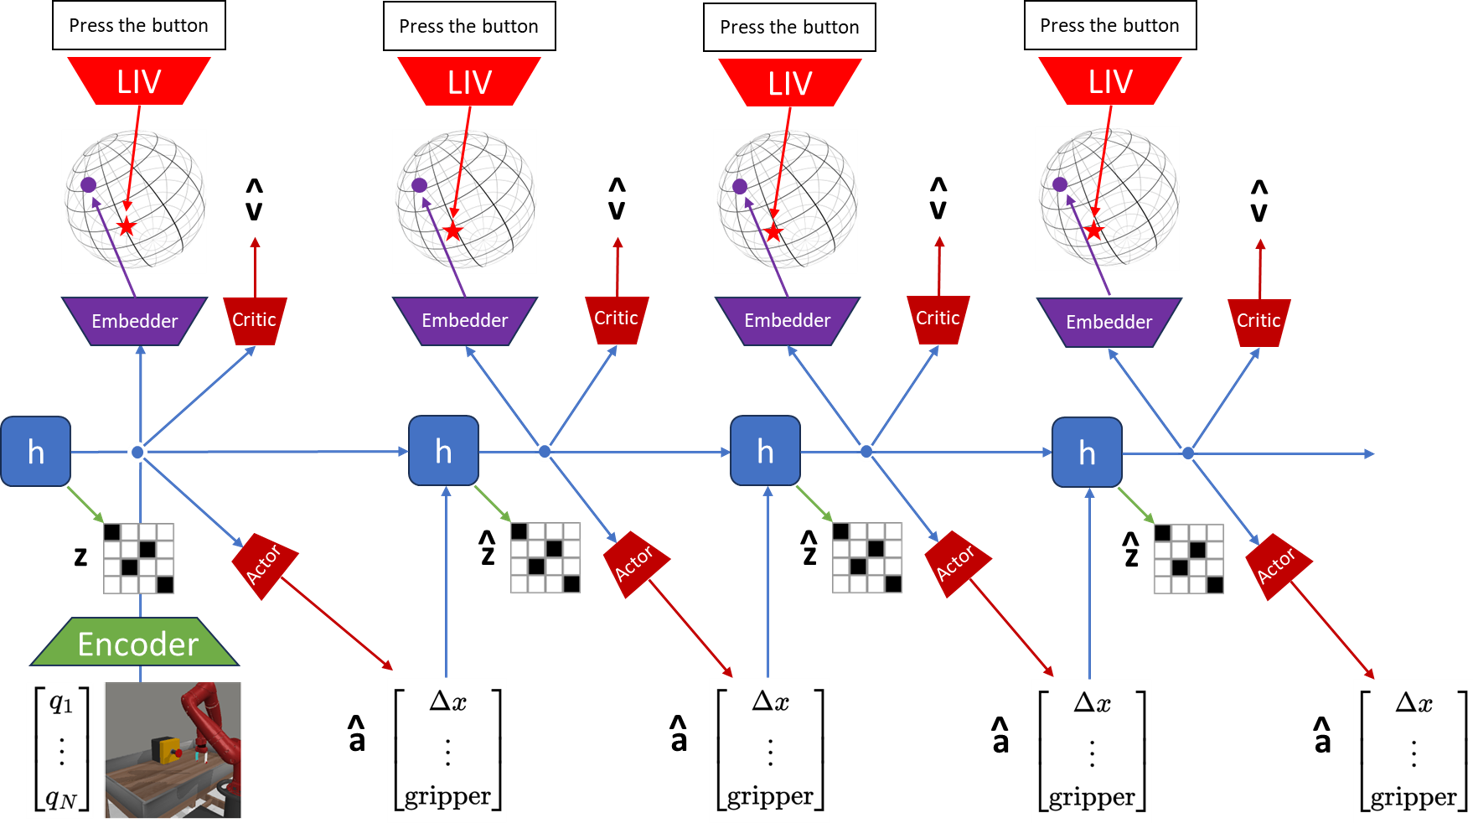
\includegraphics[width=0.6\linewidth]{actor critic agent.png}
    \caption{Actor Critic agent}
    \label{fig:Actor Critic agent}
\end{figure}

\subsection{Sampling-based MPC Agent with LIVerse}
We propose a new form of RFM that leverages LIVerse within a sampling-based model predictive control (MPC) framework \autoref{fig:MPC agent}. Unlike conventional MPCs that use a world model merely as a simulator, our approach uses LIVerse both as a simulator and a semantics-aware \textit{task interpreter}, providing reward functions. As a result, VLM based zero-shot reward model directly transfers to zero-shot policy. 

In this section, we assume the same cosine similarity reward function as the previous actor critic agent, and in the next section, we extend the reward function to the delta score function for step-wise planning.

During action selection, we employ the Cross-Entropy Method (CEM) to optimize action sequences that maximize expected similarity with the target embedding over the planning horizon. In addition to CEM, other MPC methods such as MPPI can also be applied. This MPC approach enables zero-shot generalization to new tasks.

Because of its model-predictive nature, this agent requires no training for policy. Also, task objectives can be changed at runtime in highly flexible manner. In addition, sampling-based MPC allows integration of complex physical constraints, which are crucial for real-world robotics. Furthermore, parameters such as the number of samples, noise scale, planning horizon, and constraint penalties can be adjusted to modulate behavior styles.
\begin{figure}[htbp]
    \centering
    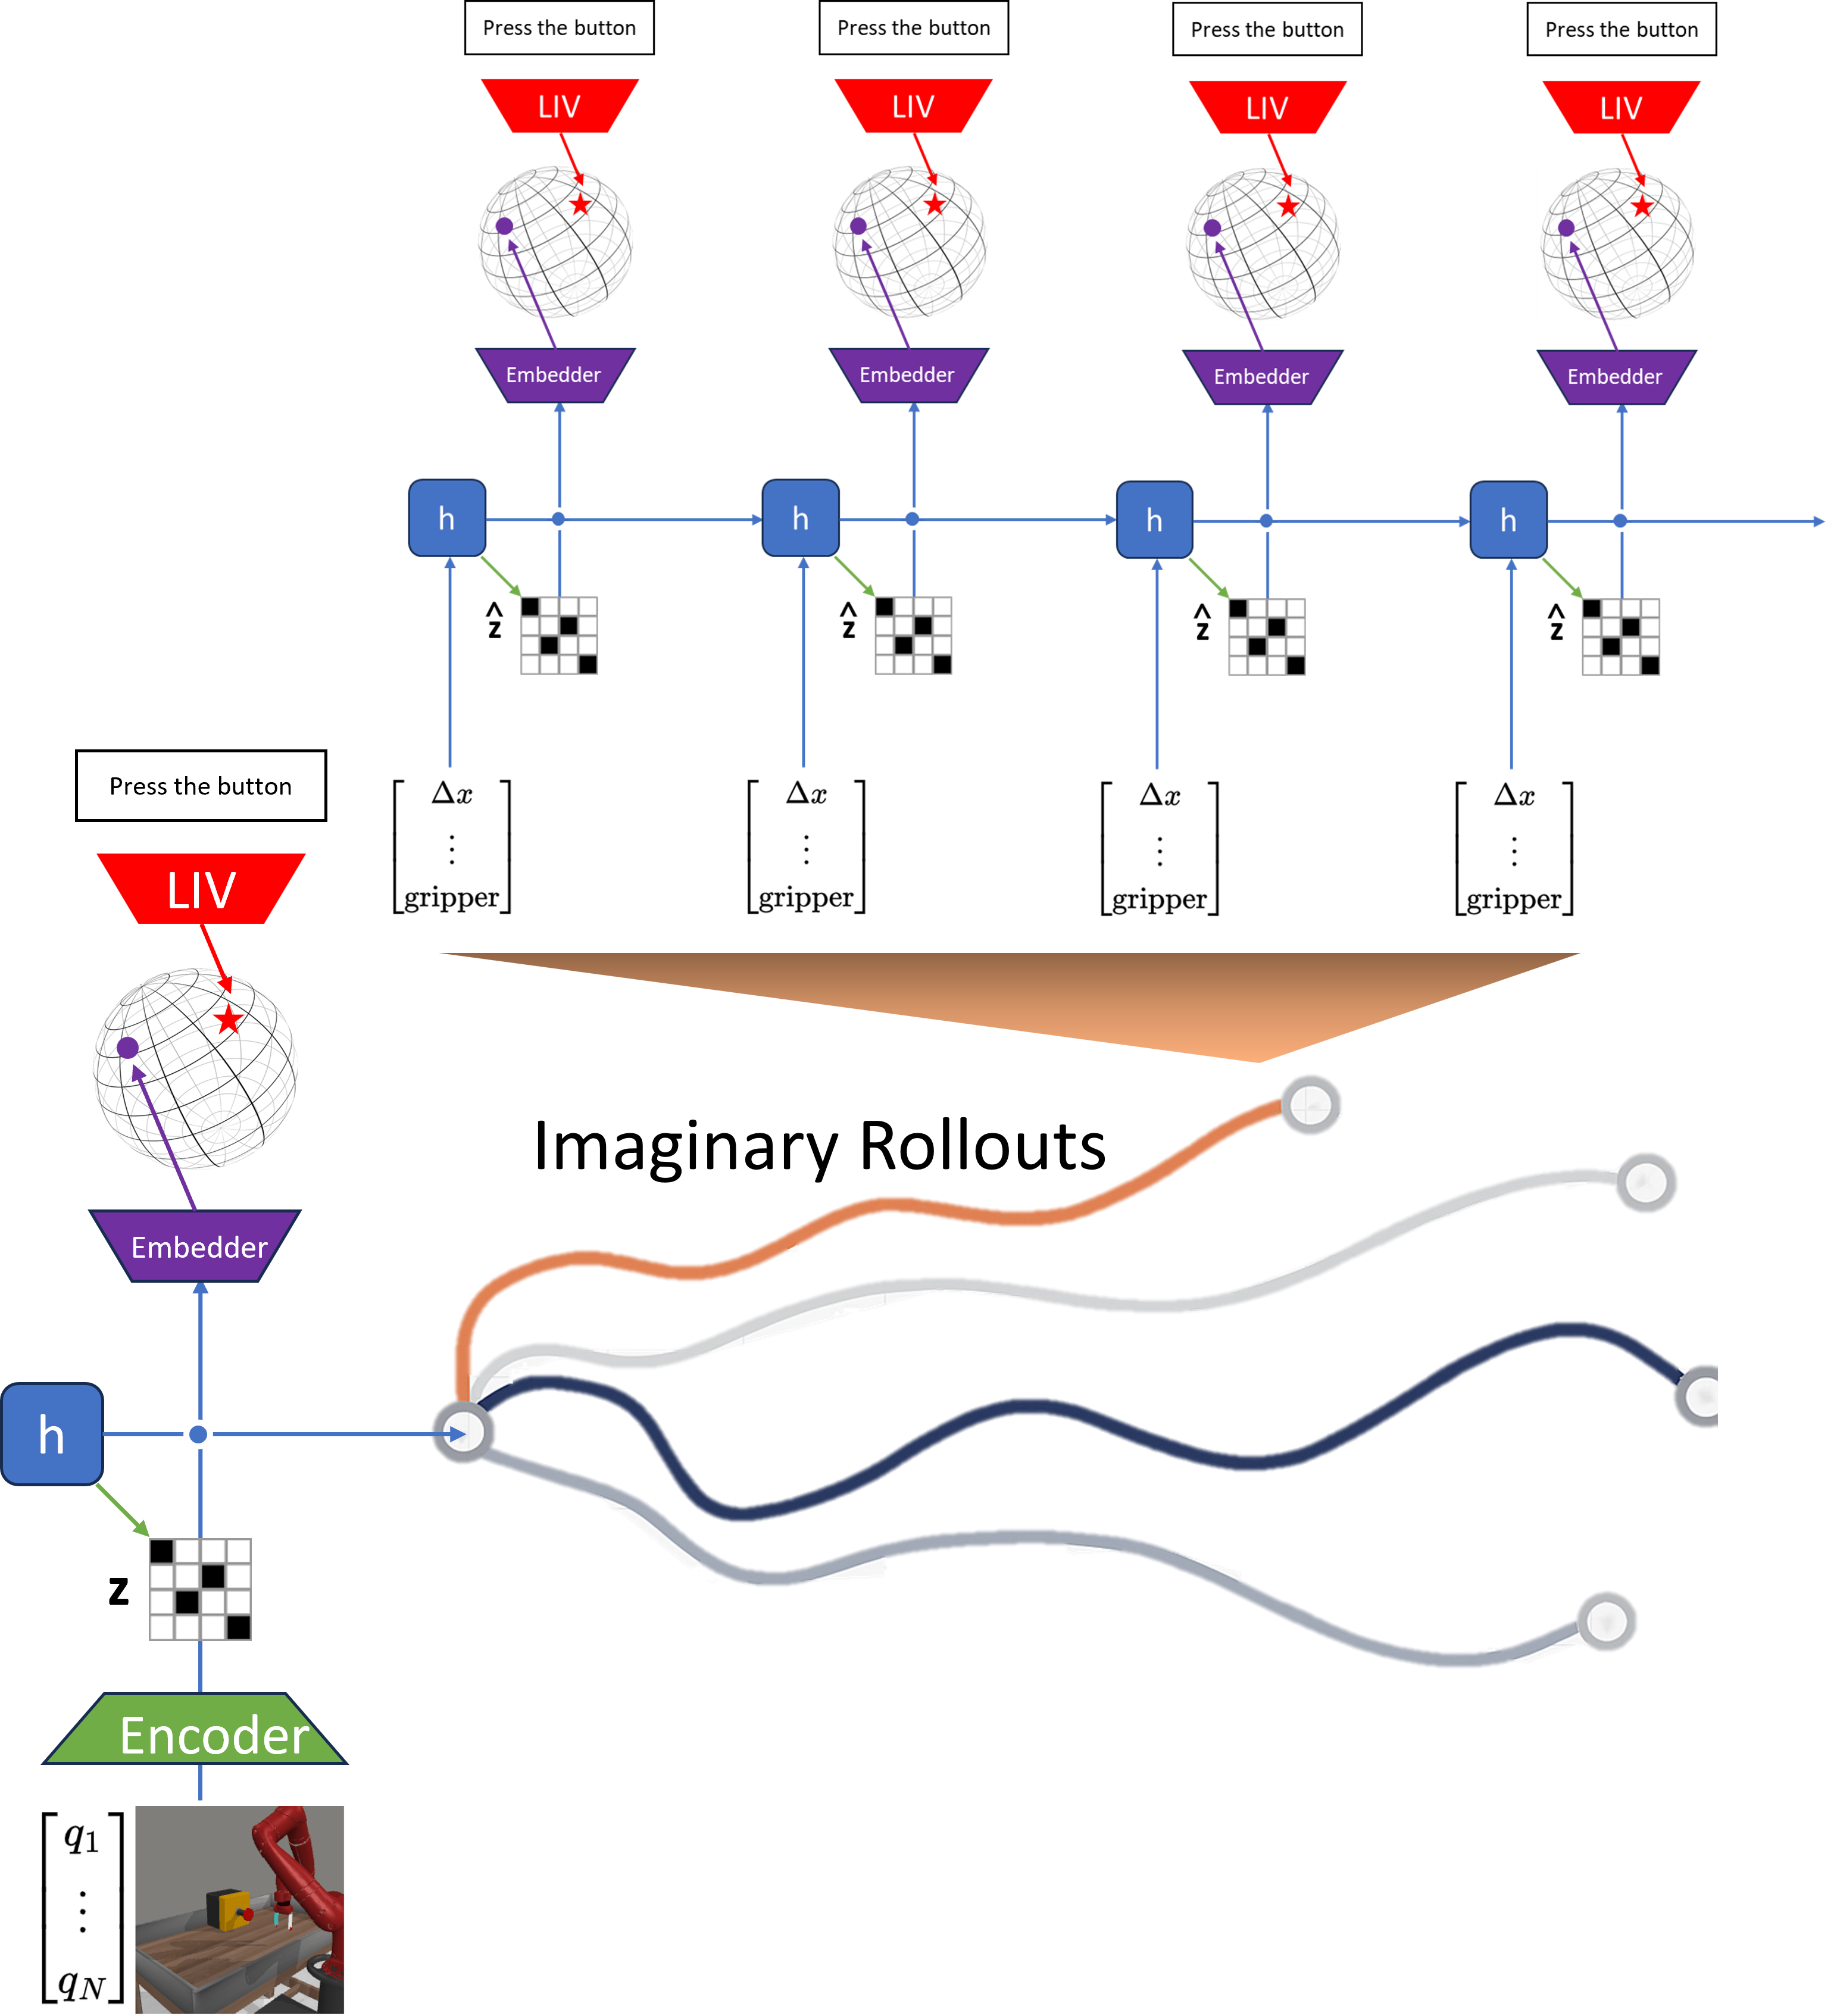
\includegraphics[width=0.45\linewidth]{MPC agent.png}
    \caption{Sampling based MPC agent}
    \label{fig:MPC agent}
\end{figure}

The following algorithm \autoref{alg:cem_liv} outlines MPC procedure using LIVerse-based cosine similarity rewards in latent space.

\begin{algorithm}
\caption{Sampling based MPC (CEM) with LIVerse}
\label{alg:cem_liv}
\begin{algorithmic}[1]
\State\textbf{Input:} Planning horizon $H$, optimization iterations $I$, number of candidates $J$, number of top candidates $K$, LIV language encoder $\mathrm{LIV}_L(l)$
\State Initialize action sequences $q(a_{t:t+H}) \leftarrow \mathcal{N}(\mathbf{0}, \mathbf{I})$
\For{$i = 1$ to $I$}
    \For{$j = 1$ to $J$}
        \State Sample $a_{t:t+H}^{(j)} \sim q(a_{t:t+H})$
        \State Initialize latent $(h_t^{(j)}, z_t^{(j)}) \sim q(h_t, z_t \mid o_{1:t}, a_{1:t-1})$
        \For{$\tau = t+1$ to $t+H+1$}
            \State Predict $(h_\tau^{(j)}, z_\tau^{(j)}) \sim p(h_\tau, z_\tau \mid h_{\tau-1}^{(j)}, z_{\tau-1}^{(j)}, a_{\tau-1}^{(j)})$
            \State Predict LIV image embedding $\hat{e}_{I_\tau}^{(j)}$ from $(h_\tau^{(j)}, z_\tau^{(j)})$
        \EndFor
        \State Compute reward:
        \[
        R^{(j)} = \sum_{\tau = t+1}^{t+H+1} \frac{\mathrm{LIV}_L(l) \cdot \hat{e}_{I_\tau}^{(j)}}{\|\mathrm{LIV}_L(l)\| \cdot \|\hat{e}_{I_\tau}^{(j)}\|}
        \]
    \EndFor
    \State Select indices $\mathcal{K}$ of top $K$ sequences with highest $R^{(j)}$
    \State Update mean:
    \[
    \mu_{t:t+H} = \frac{1}{K} \sum_{k \in \mathcal{K}} a_{t:t+H}^{(k)}
    \]
    \State Update std:
    \[
    \sigma_{t:t+H} = \sqrt{ \frac{1}{K-1} \sum_{k \in \mathcal{K}} (a_{t:t+H}^{(k)} - \mu_{t:t+H})^2 }
    \]
    \State Update distribution:
    \[
    q(a_{t:t+H}) \leftarrow \mathcal{N}(\mu_{t:t+H}, \mathrm{diag}(\sigma_{t:t+H}^2))
    \]
\EndFor
\State \textbf{return} first action mean $\mu_t$
\end{algorithmic}
\end{algorithm}

\section{Delta-score based Reward for Step-wise Planning}

\subsection{Step-wise Planning}
While VLM-based rewards enable flexible task specification through natural language, they are inherently limited to behave as \textit{fixed point tracking}, optimizing actions to minimize distance in the embedding space to a fixed goal vector. However, good trajectories that successfully performs a task are often not the optimal path of the shortest distance.
So, cosine-similarity reward becomes problematic as the trajectory non-linearity increases in complex tasks. In such cases, agents often fail to explore alternate or curved paths in embedding space that are necessary due to physical or task constraints. 
To overcome these limitations, we need a step-wise planning that decomposes complex task into several subtasks, and this step-by-step goal setting increases the linearity of each sub-trajectory.

\subsection{Delta-score based reward}
However, if the target embeddings are changed for each subtask, the reward scale itself changes for each subtask, which causes avoiding to move to the next subtask. To escape from this local minima, we proposes the delta-score that measures the \textit{incremental improvement in similarity} rather than absolute similarity itself. At each timestep, the reward is computed as:
\begin{equation}
r_t = \Delta \text{Score}_t = 
\frac{
    \mathrm{LIV}_L(l) \cdot \hat{e}_{I_{t}}
}{
    \|\mathrm{LIV}_L(l)\| \cdot \|\hat{e}_{I_{t}}\|
}
-
\frac{
    \mathrm{LIV}_L(l) \cdot \hat{e}_{I_{t-1}}
}{
    \|\mathrm{LIV}_L(l)\| \cdot \|\hat{e}_{I_{t-1}}\|
}
\end{equation}
This reward formulation naturally supports \textit{step-wise planning} by allowing the system to decompose complex tasks into intermediate sub-goals, where each sub-task is rewarded based on its own progress.
Now, our full architecture \autoref{fig:Whole Architecture of LIVerse based MPC agent} can incorporate a high-level hierarchical planner that sequences sub-tasks through texts or images or latent representations, with LIVerse-bas  `ed MPC.
\begin{figure}
    \centering
    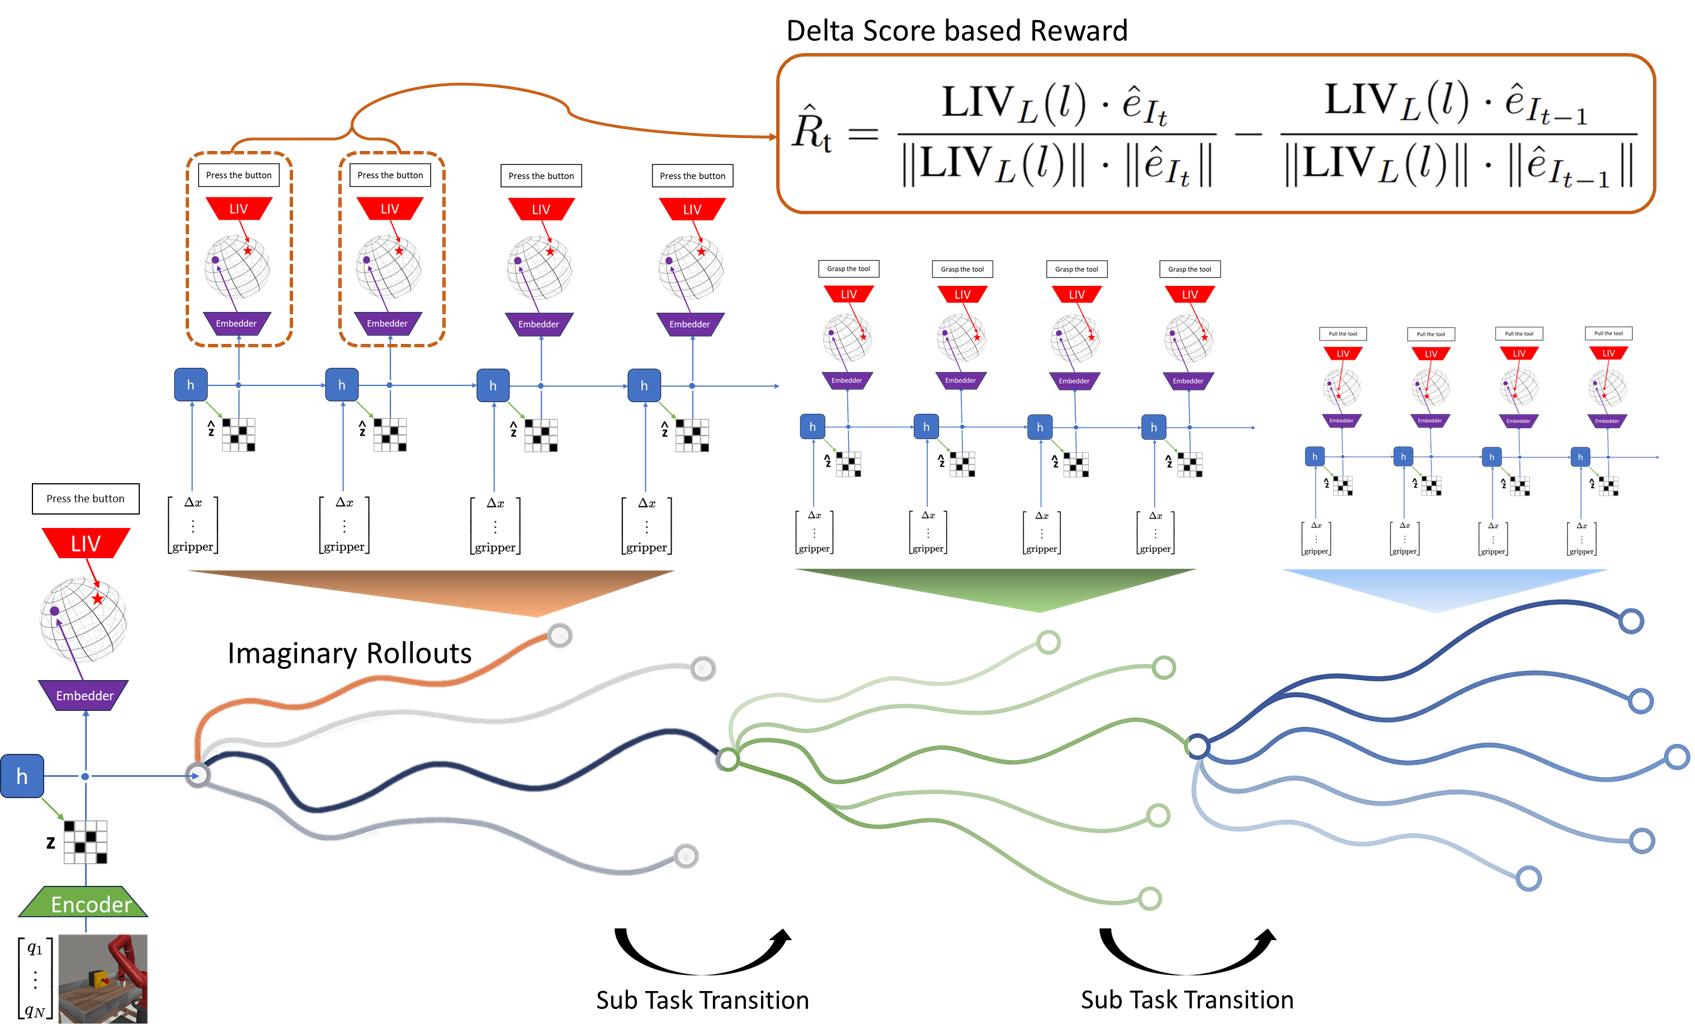
\includegraphics[width=1\linewidth]{sampling based MPC agent.png}
    \caption{Whole Architecture of LIVerse based MPC agent}
    \label{fig:Whole Architecture of LIVerse based MPC agent}
\end{figure}

\section{Experiments}

\subsection{Meta-World Environment}
\begin{itemize}
\item \textbf{Task}: For our experiments, we utilized tasks from the Meta-World benchmark, which provides a diverse set of robotic manipulation challenges. Specifically, we focused on the ML1 button press, drawer close, window close, lever pull task. In this study, each episode was set to 500 timesteps, corresponding to 5 seconds in the real world, and performance was evaluated every 20 episodes. 
\item \textbf{Observation Space}: The observation space in our implementation consists of two main components: visual observations (224 x 224 x 3 RGB image) and robot+object states (39-dimensional vector), forming the complete observation used in this work.
\item \textbf{Action Space}: The action space is a 4-dimensional continuous vector comprising the 3D displacement of the Sawyer robot’s end-effector and a normalized scalar controlling the gripper’s open/close torque. Each action dimension is normalized to the range [−1,1].
\item \textbf{Dynamics}: The simple dynamics where the action directly corresponds to a delta state enable the cosine similarity-based reward to more explicitly induce fixed-point tracking behavior. This property is one of the reasons we chose Meta-World as our environment. 
\end{itemize}

\subsection{Selecting Camera view and Text description}
To evaluate the impact of camera perspectives and text description on performance, we implemented an rule-based oracle policy with access to perfect state information. This policy was then evaluated under various camera configurations and text descriptions to assess how they affect the VLM-Rewards during episodes. 
Although not a perfect ego-centric view, our findings suggest that camera id = 1 view generally provides best performance, being free from occlusions caused by the robot arm and allowing clear observation of changes in the image frame. \autoref{fig:right-image}
For task representations using text descriptions, both the magnitude of the similarity reward itself and its positive correlation with task progression are crucial. Unfortunately, none of the text descriptions we tested demonstrated a consistently good reward score trend. \autoref{fig:left-image}Using subjects like "robot" or "agent" was more effective than omitting the subject or using terms such as "arm" or "hand." Among verb expressions like "click," "push," "press," and "reach," the verb "push" yielded the highest reward scores and showed a clear upward trend aligned with button-press task progress. However, even the best-performing description, \textit{"Robot pushes button,"} did not achieve performance levels sufficient for practical application in model-based reinforcement learning. 
But we found that the goal image for target embedding provides both high rewards and a clear positive trend aligned with task progression. Notably, this performance was maintained even for AI-generated images similar to the original image, rather than relying solely on the real rendered-image itself.

Therefore, for subsequent experiments, we set the target embedding to be the LIV image embedding vector of the goal image. Since this embedding remains within the shared vision-and-language embedding space, it does not introduce any issues related to the model architecture proposed in this study.
\begin{figure}[htbp]
    \centering
    \begin{minipage}[b]{0.48\linewidth}
        \centering
        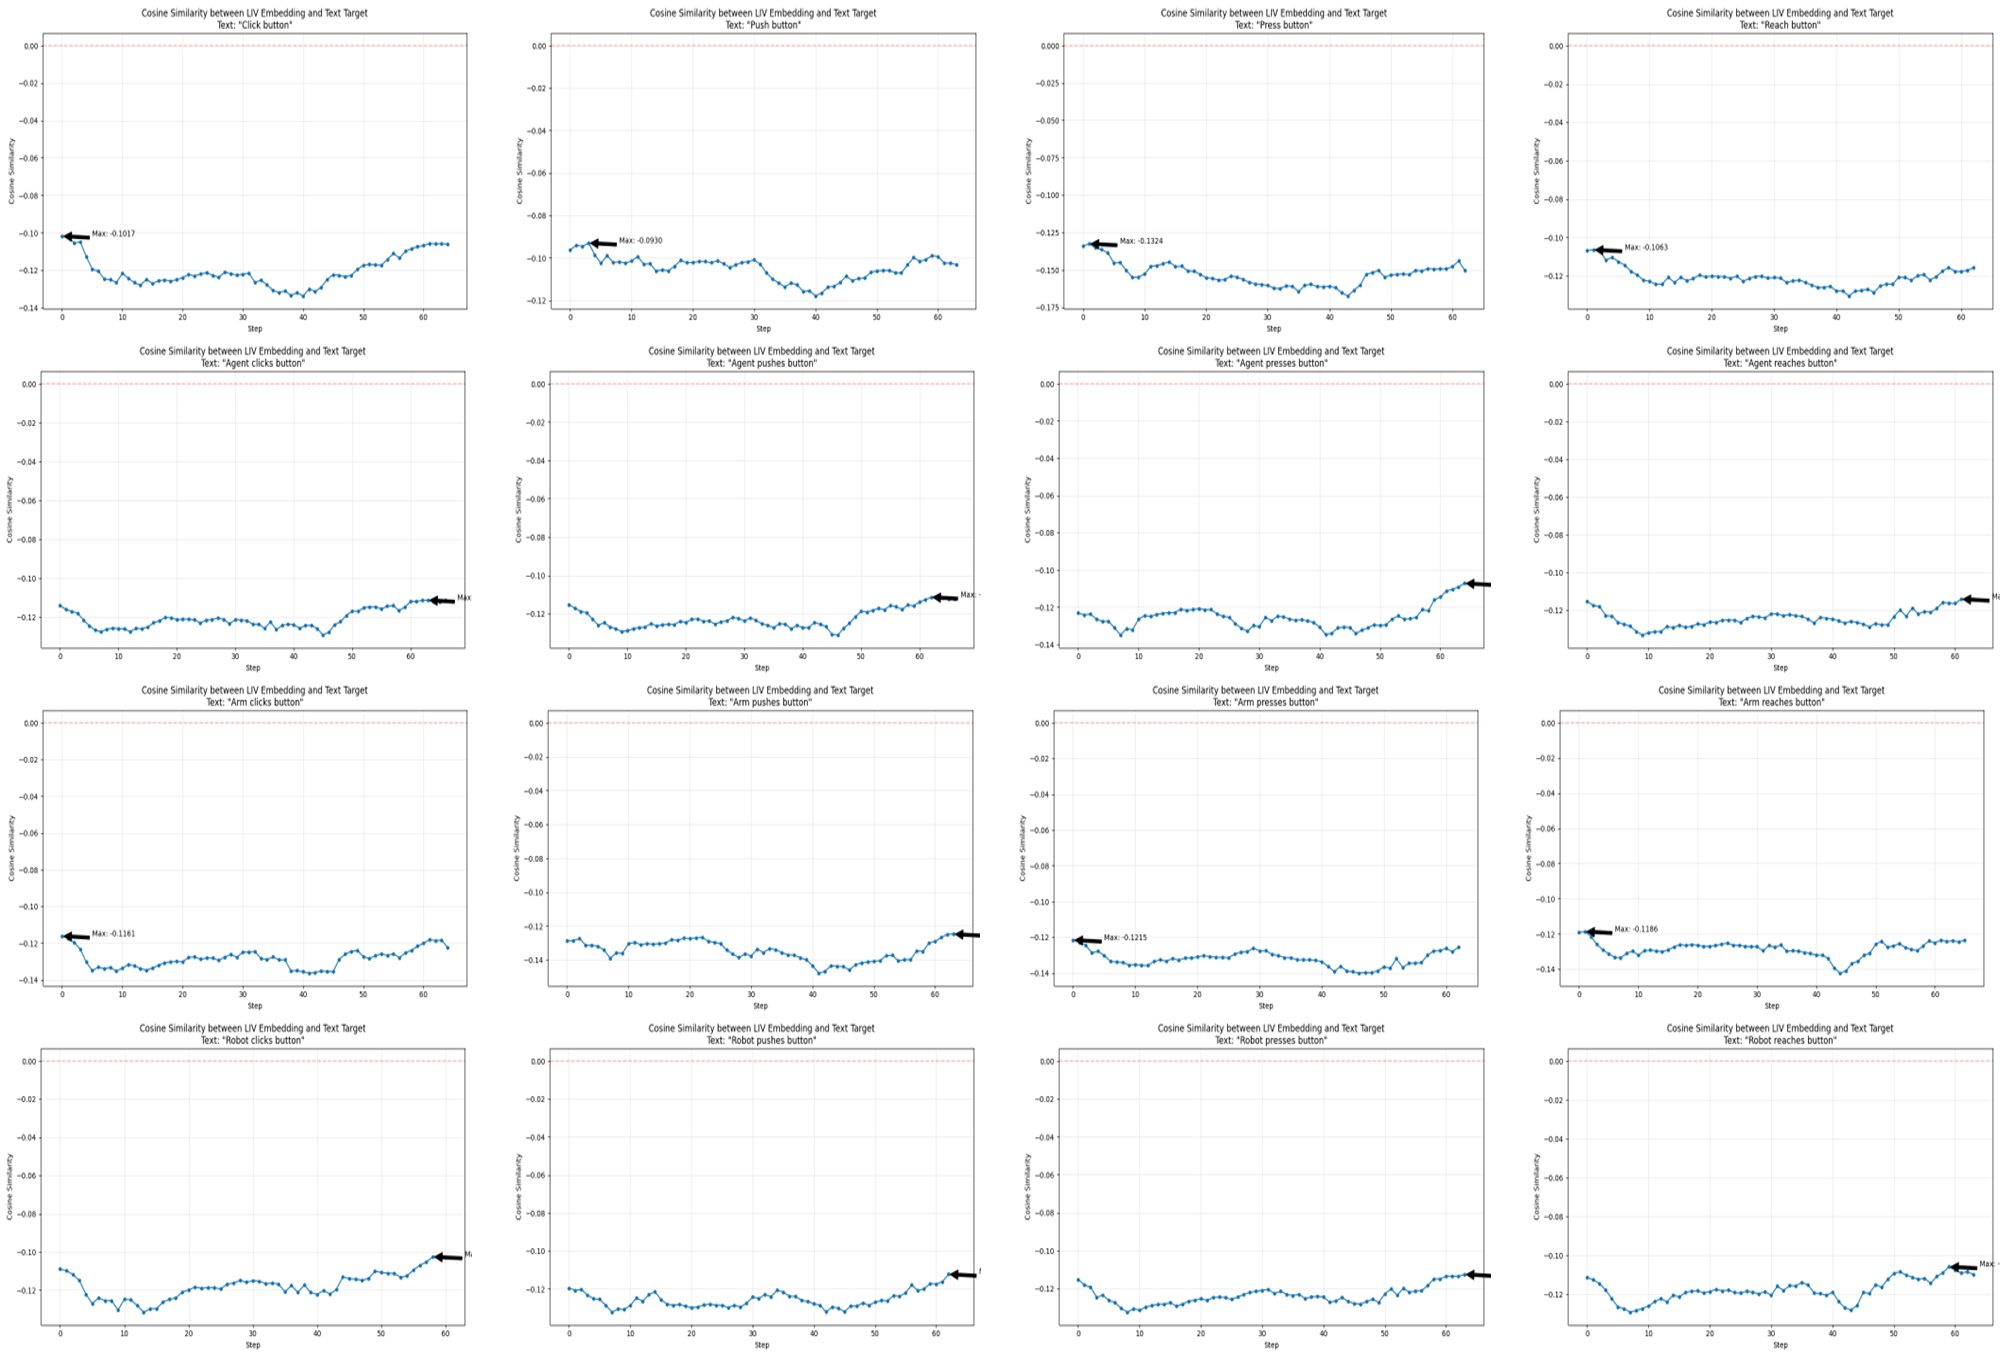
\includegraphics[width=\linewidth]{text description.png}
        \caption{Rewards based on various texts}
        \label{fig:left-image}
    \end{minipage}
    \hfill
    \begin{minipage}[b]{0.4\linewidth}
        \centering
        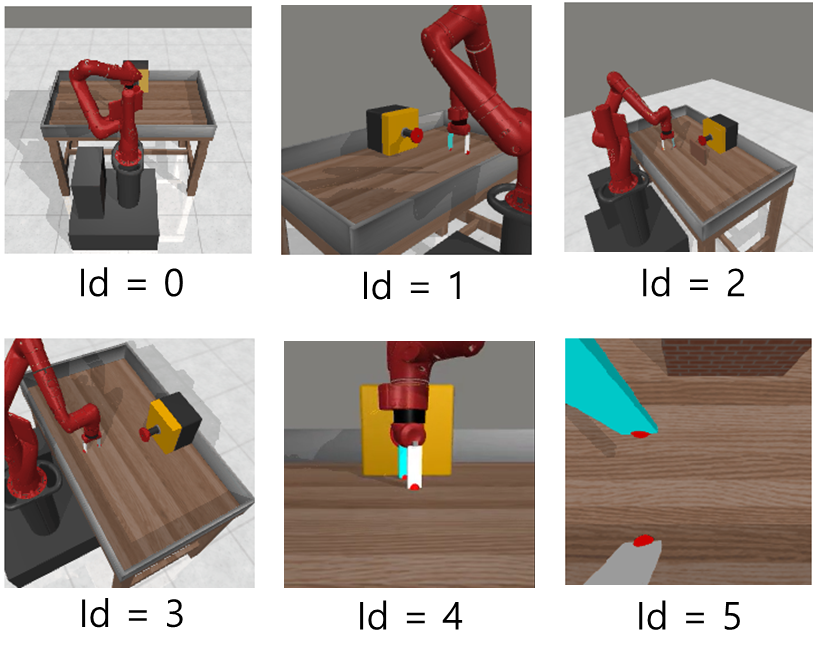
\includegraphics[width=\linewidth]{camera view.png}
        \caption{Various camera views}
        \label{fig:right-image}
    \end{minipage}
\end{figure}

\subsection{Learning process of LIVerse}
The \autoref{fig:Image Reconstruction} shows selected results of video reconstruction after 20, 40, and 60 episodes, respectively. Visual reconstruction quality, assessed through the world model's decoder outputs, shows clear improvement over training. Initial reconstructions appear blurry and lack detail, but as the model interacts more with the environment, the reconstructions progressively improve, becoming sharper and more accurate in capturing the robot’s configuration and the state of the environment. This visual fidelity is crucial for effective imagination-based learning in the Dreamer framework.

\subsection{Transfer Learning of World Model}
The \autoref{fig:Transfer learning} plots the ratio of model losses during two separate LIVerse training processes over the course of episodes. The first training was the initial world model learning in the button press environment without any pretraining. The second training started from the LIVerse model trained on the button press environment and continued training in the drawer close environment.
From the graph, we observe an overall decrease of model loss in second training. Notably, the model loss ratio is very low in the early episodes, demonstrating the few-shot learning capability of the model, which can learn quickly with minimal interaction. After approximately 160 episodes, the ratio approaches near 1, but it is due to the model losses in both training phases have sufficiently converged.
\begin{figure}[htbp]
    \centering
    \begin{minipage}[b]{0.48\linewidth}
        \centering
        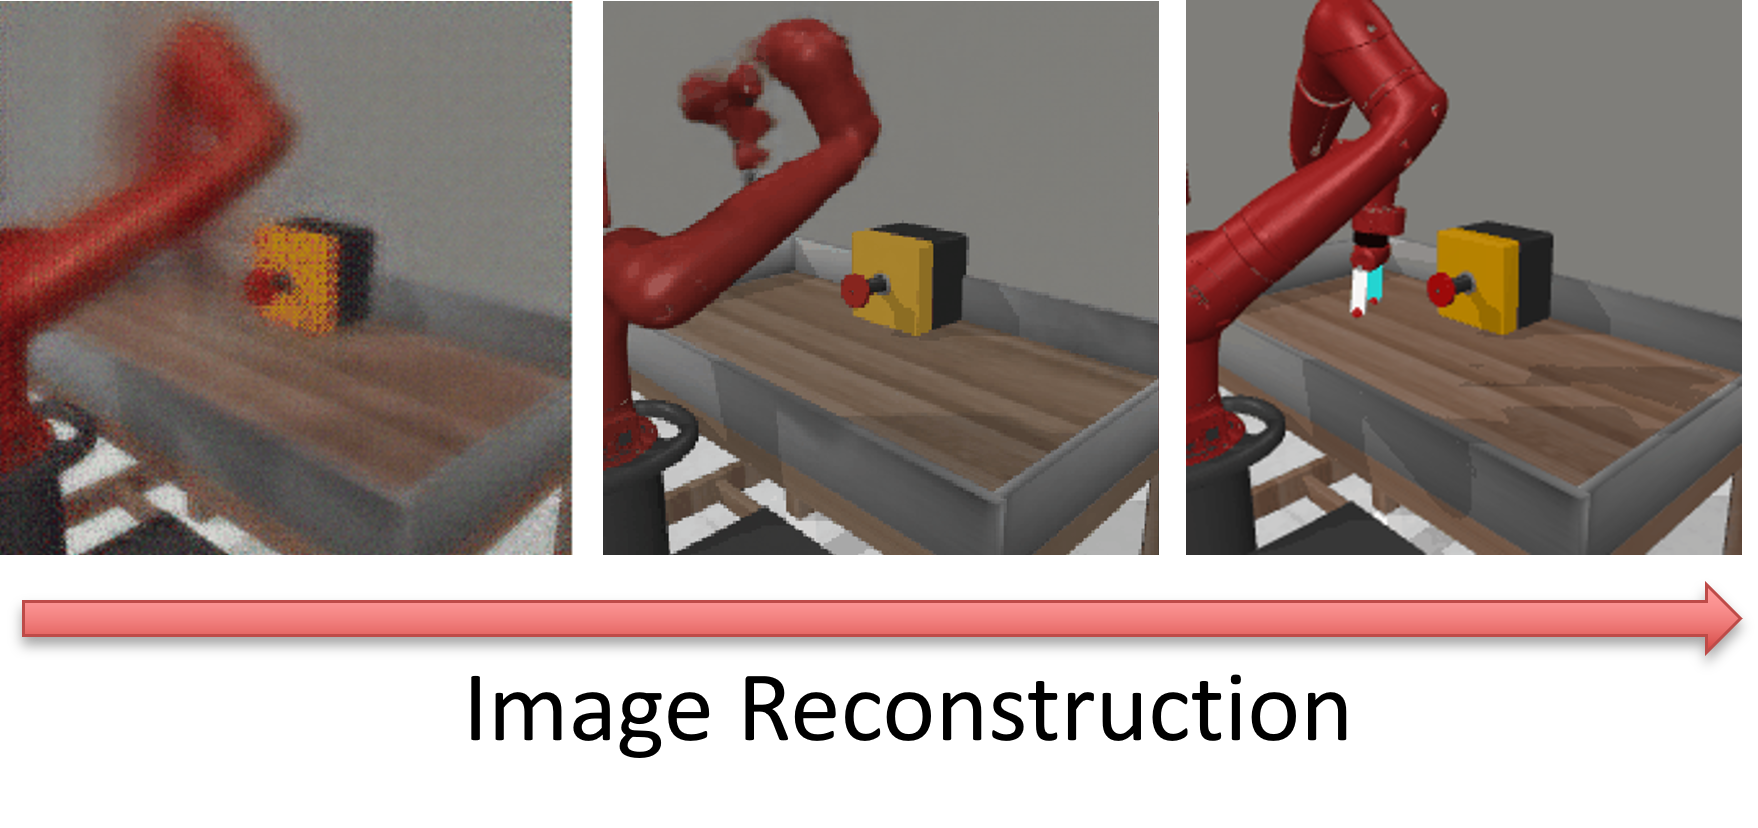
\includegraphics[width=\linewidth]{image reconstruction.png}
        \caption{Image Reconstruction}
        \label{fig:Image Reconstruction}
    \end{minipage}
    \hfill
    \begin{minipage}[b]{0.48\linewidth}
        \centering
        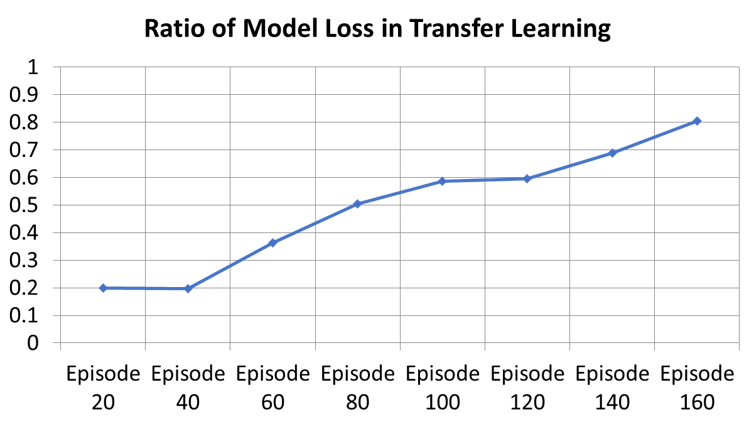
\includegraphics[width=\linewidth]{graph_transfer learning.png}
        \caption{Transfer learning of LIV}
        \label{fig:Transfer learning}
    \end{minipage}
\end{figure}

\subsection{Zero-Shot Policy performance of LIVerse based MPC}
The LIVerse used in this experiment was trained in the button press environment, with the Actor-Critic version agent utilizing an entropy-based intrinsic reward without any VLM-rewards. While the actor-critic training did not utilize the VLM reward, the prediction module of the world model was, of course, trained using the LIV embeddings. Thus, it is a task-agnostic world model that has only experienced the button box environment.
Using this LIVerse world model within an MPC framework, we evaluated four environments/tasks: button press, drawer close, window close, and lever pull. The zero-shot policy performance results are shown in the following \autoref{fig:Zero-shot policy performance}. While the success rates for window close and lever pull were low, the model achieved a perfect success rate on the button press task and mostly succeeded on drawer close as well. The \autoref{fig:Button press task} shows the similarity score and difference reward over 200 timesteps for a successful trajectory in the button press task.

Additionally, although the robot was unable to fully press and insert the button, we  found that MPC that uses AI-generated image \label{fig:AI} instead of real rendered image was still able to touch the button. As a result, by simply changing the goal image, the agent was able to partially succeed in adapting to new tasks within zero-shot manner. 
\begin{figure}[htbp]
    \centering
    \begin{minipage}[b]{0.48\linewidth}
        \centering
        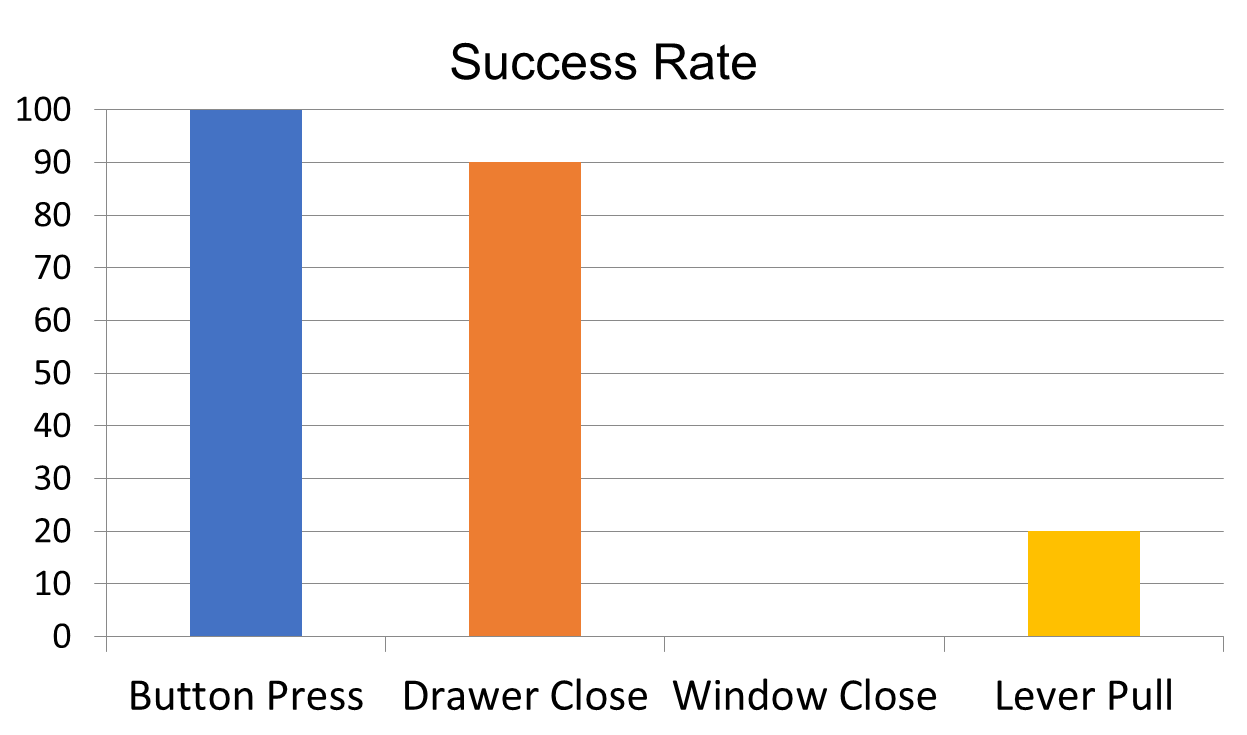
\includegraphics[width=\linewidth]{graph_zero shot policy.png}
        \caption{Zero-shot policy performance}
        \label{fig:Zero-shot policy performance}
    \end{minipage}
    \hfill
    \begin{minipage}[b]{0.3\linewidth}
        \centering
        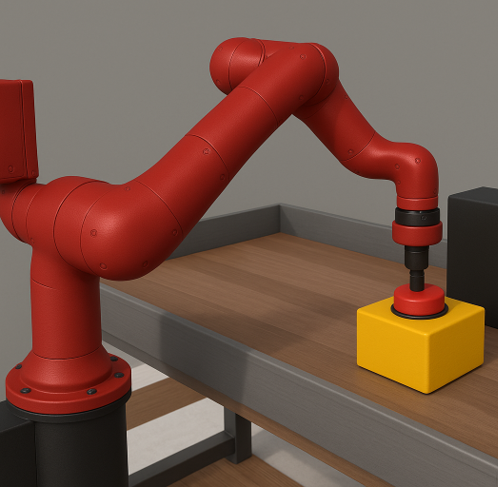
\includegraphics[width=\linewidth]{ai.png}
        \caption{AI generated goal image}
        \label{fig:AI}
    \end{minipage}
\end{figure}

\begin{figure}[htbp]
    \centering
    \begin{minipage}[b]{0.48\linewidth}
        \centering
        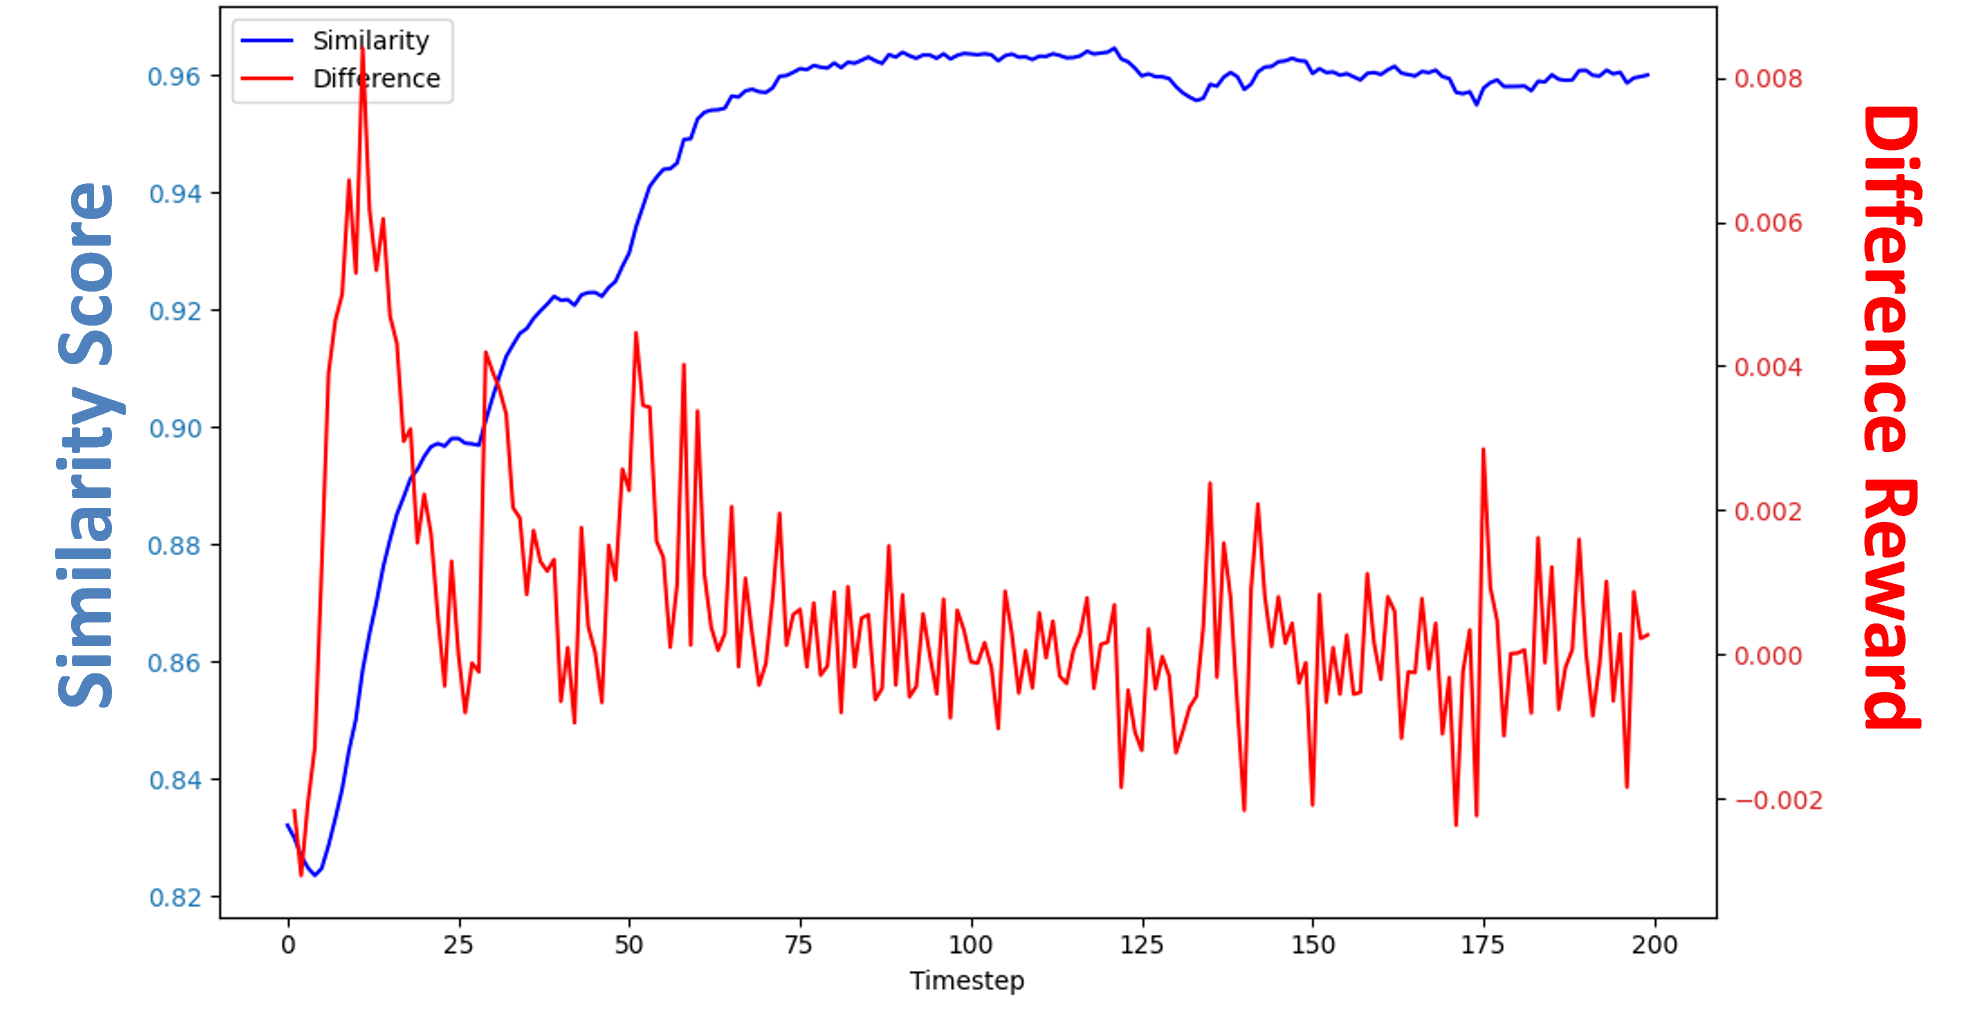
\includegraphics[width=\linewidth]{graph_button press.png}
        \caption{Button press task}
        \label{fig:Button press task}
    \end{minipage}
    \hfill
    \begin{minipage}[b]{0.42\linewidth}
        \centering
        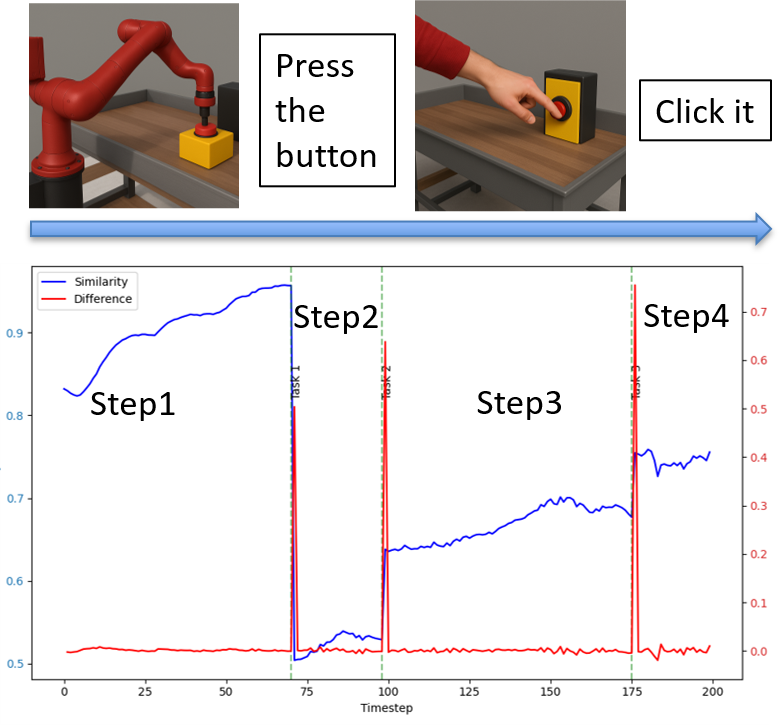
\includegraphics[width=\linewidth]{step-wise planning.png}
        \caption{Multi-modal sub tasks}
        \label{fig:Multi-modal}
    \end{minipage}
\end{figure}

\subsection{Step-wise planning with Delta-score based reward}
Finally, we conducted three complex task experiments using the proposed LIVerse-based MPC agent with step-wise planning \autoref{fig:Whole Architecture of LIVerse based MPC agent}. In this experiment, the task transition condition was rule-based, checking whether the difference reward remained below a certain threshold for a specified number of consecutive timesteps.
\begin{enumerate}
    \item A periodic task of pressing and releasing a button,
    \item A curved trajectory task where the arm moves left before pressing the button,
    \item A step-wise planning task involving a mixture of multi-modal task representations, such as different image styles and text descriptions.
\end{enumerate}
The subtasks used and the results for each experiment are shown in the following \autoref{fig:Multi-modal},\autoref{fig:Button press task},\autoref{fig:Multi-modal}. The results show that at each subtask transition, there is a sharp change in the reward scale. Therefore, if only the traditional cosine similarity reward is used without employing the delta-score based reward model, the local minima problem arising during subtask transitions cannot be resolved. Moreover, the approach is agnostic to the modality used to generate the target embedding, allowing tasks to be defined across diverse modalities.

\begin{figure}[htbp]
    \centering
    \begin{minipage}[b]{0.47\linewidth}
        \centering
        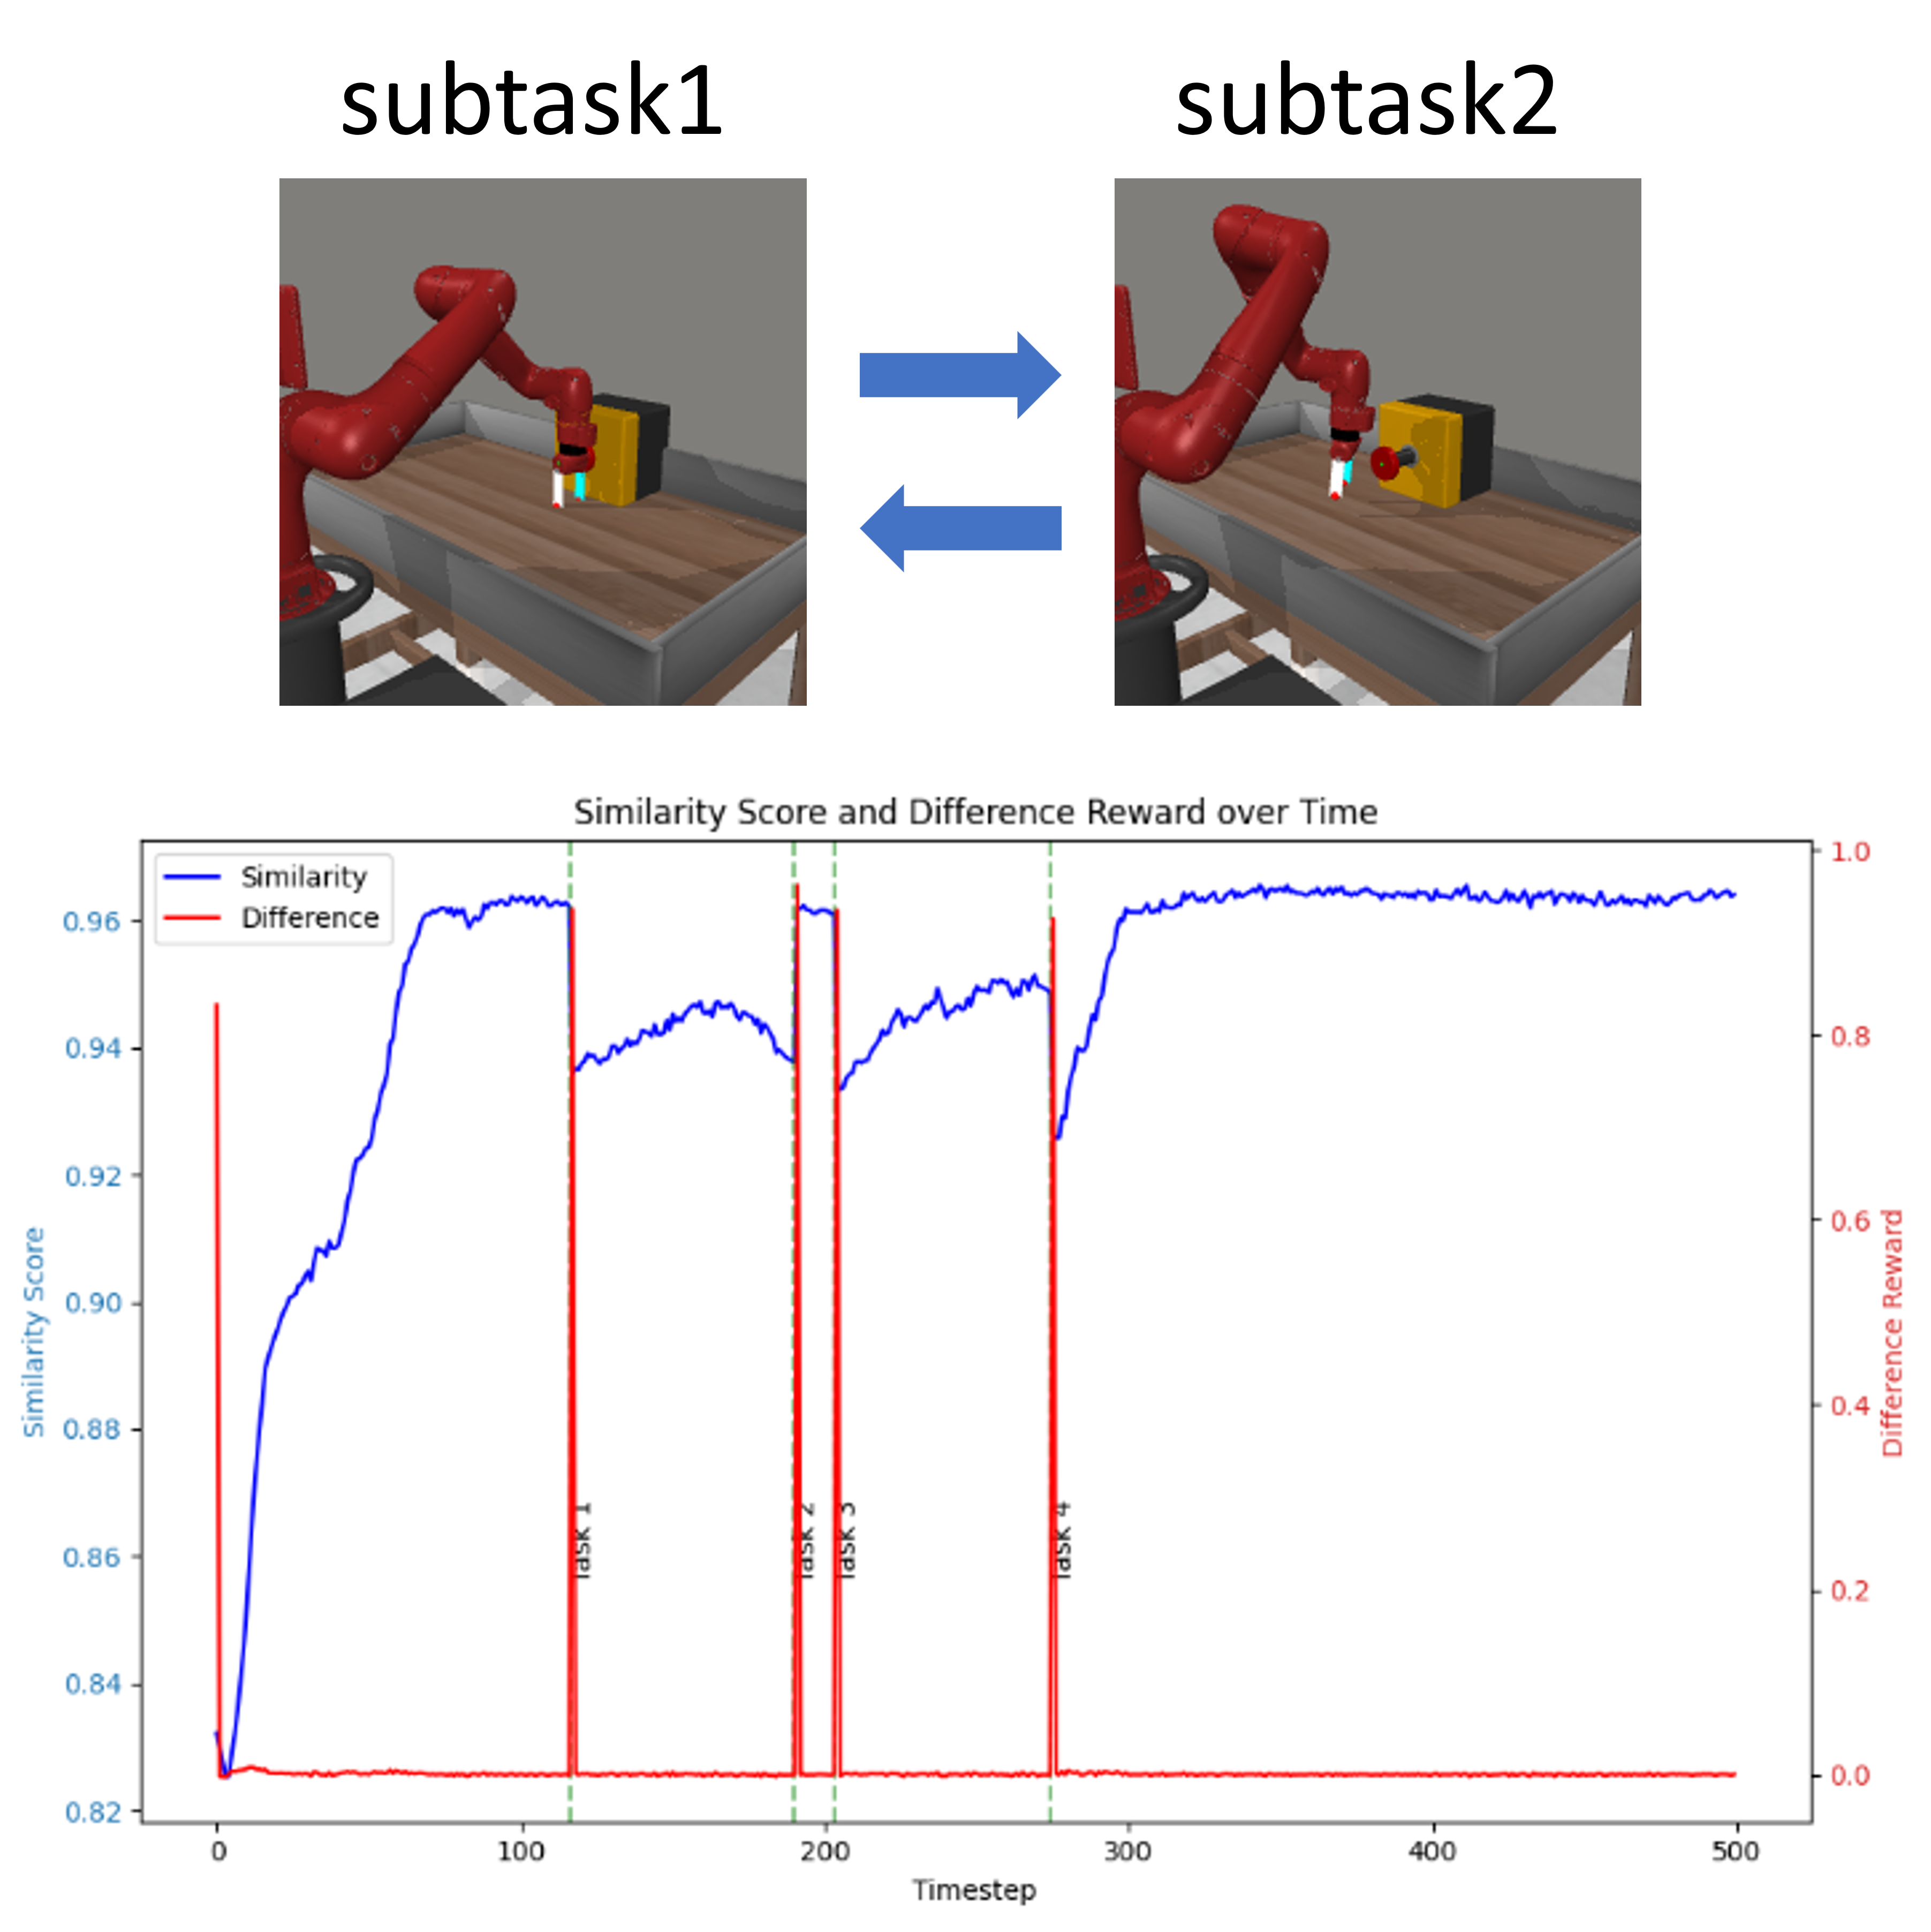
\includegraphics[width=\linewidth]{cycle.png}
        \caption{Periodic task}
        \label{fig:cycle}
    \end{minipage}
    \hfill
    \begin{minipage}[b]{0.48\linewidth}
        \centering
        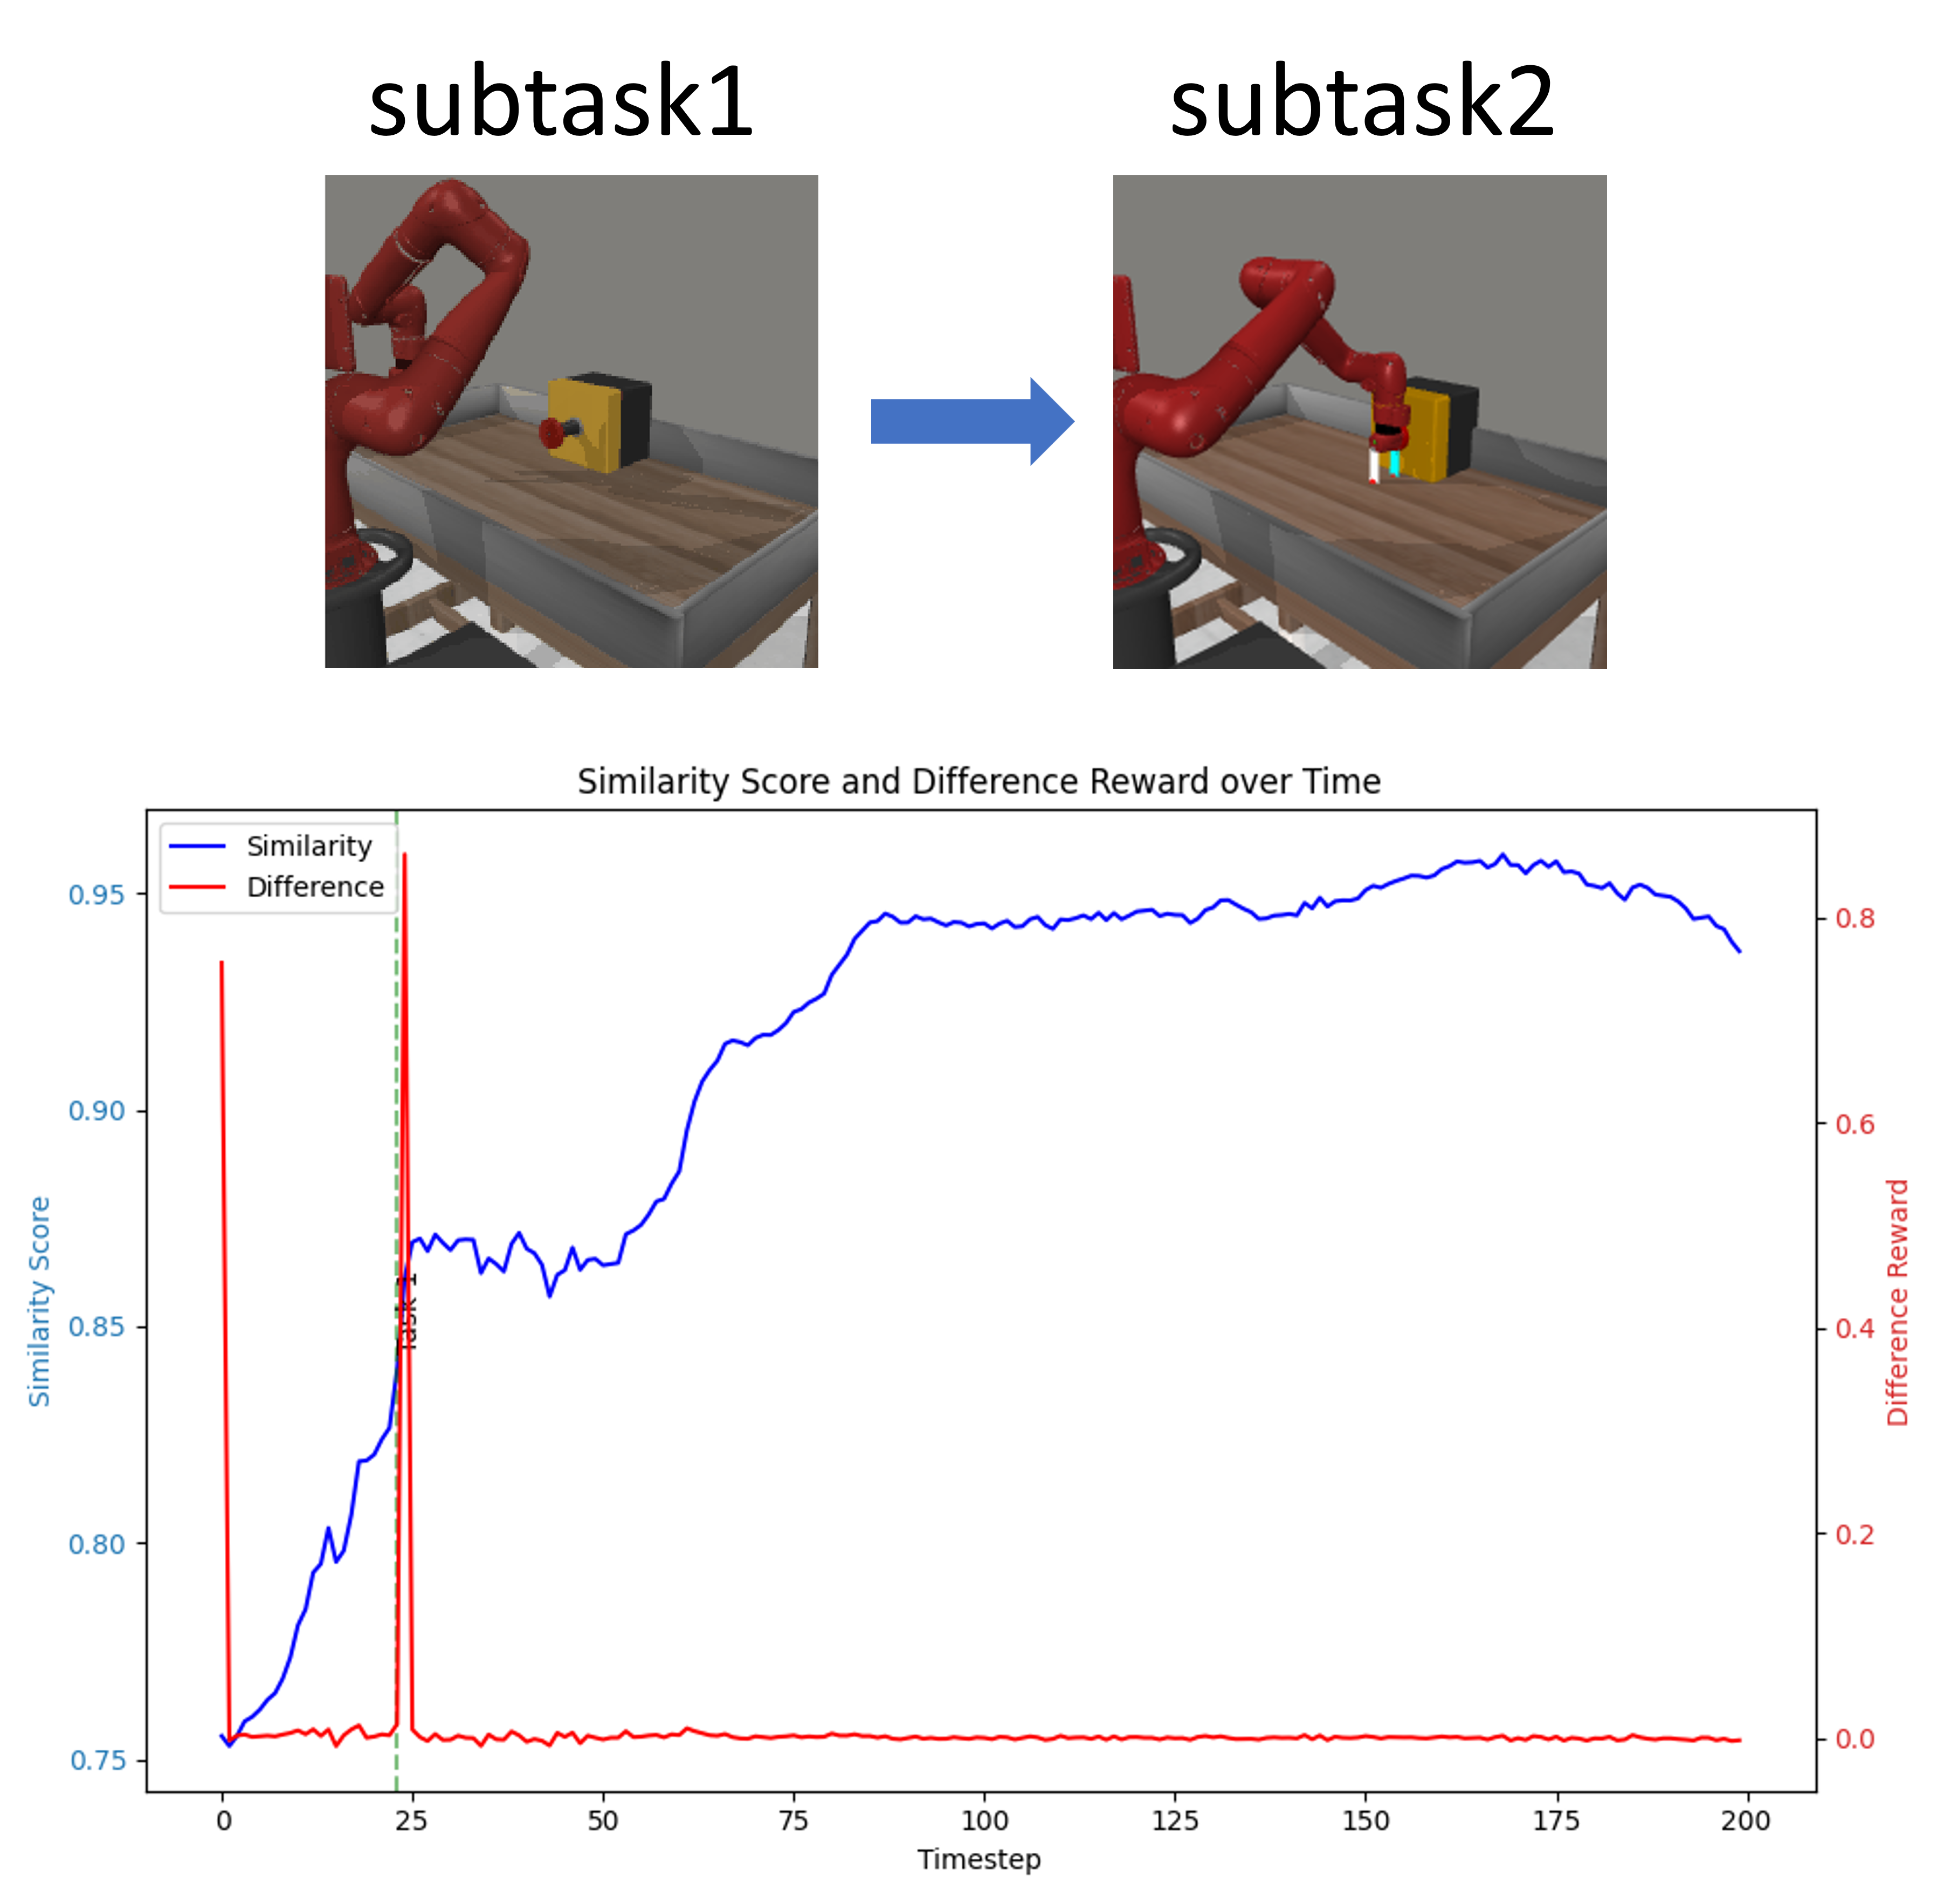
\includegraphics[width=\linewidth]{curve.png}
        \caption{Curved trajectory task}
        \label{fig:curve}
    \end{minipage}
\end{figure}

\section{Conclusions and Future works}
In this paper, we present \textbf{LIVerse}, a novel World Foundation Model that integrates vision-language semantics and robot dynamics into a unified latent space. By leveraging pretrained vision-language models not as direct action generators but as dense, transferable reward models, LIVerse-based Reinforcement Learning overcomes key limitations of current Robot Foundation Models, which primarily rely on imitation learning and generative policies.

We explored two main agent architectures on top of LIVerse: a Dreamer-style Actor-Critic agent and a PlaNet-style sampling-based MPC agent. The former benefits from sample efficiency, while the latter enables real-time zero-shot policy execution. Importantly, our proposed delta-score based reward function supports step-wise planning enabling the decomposition of complex tasks into subtasks and improving performance in long-horizon scenarios.

Extensive experiments on the Meta-World benchmark validate the proposed system. Our results show that the LIVerse framework effectively bridges the gap between model-based reinforcement learning and vision-language reward model. This design unlocks new possibilities for generalizable and scalable robot control systems that are capable of adapting to unseen tasks and environments. 

Due to the performance limitations of the VLM model, LIV used in this study, it was difficult to effectively evaluate the language-conditioned policy. In future work, we plan to integrate a more powerful VLM into LIVerse to address this limitation. 

\textbf{In future works}, we aim to explore several promising directions: (1) unifying multi-camera views within VLM embeddings, (2) consolidating multiple text descriptions in VLM embeddings, (3) integrating explicit robot dynamics model into the LIVerse latent space, and (4) enhancing the stepwise reward and subtask transition conditions for hierarchical planning.

% References section
\clearpage
% References section
\clearpage
\begin{thebibliography}{99}

\bibitem{planet}
Danijar Hafner, Timothy Lillicrap, Ian Fischer, Ruben Villegas, David Ha, Honglak Lee, James Davidson,
``Learning Latent Dynamics for Planning from Pixels,''
\textit{International Conference on Machine Learning}, PMLR, 2019.

\bibitem{dreamer}
Danijar Hafner, Jurgis Pasukonis, Jimmy Ba, Timothy Lillicrap,
``Mastering Diverse Domains through World Models,''
\textit{arXiv preprint arXiv:2301.04104}, 2023.

\bibitem{clip}
Alec Radford, Jong Wook Kim, Chris Hallacy, Aditya Ramesh, Gabriel Goh, Sandhini Agarwal, Girish Sastry, Amanda Askell, Pamela Mishkin, Jack Clark, Gretchen Krueger, Ilya Sutskever,
``Learning Transferable Visual Models from Natural Language Supervision,''
\textit{International Conference on Machine Learning}, PMLR, 2021.

\bibitem{r3m}
Suraj Nair, Aravind Rajeswaran, Vikash Kumar, Chelsea Finn, Abhinav Gupta,
``R3M: A Universal Visual Representation for Robot Manipulation,''
\textit{arXiv preprint arXiv:2203.12601}, 2022.

\bibitem{vip}
Yecheng Jason Ma, Shagun Sodhani, Dinesh Jayaraman, Osbert Bastani, Vikash Kumar, Amy Zhang,
``VIP: Towards Universal Visual Reward and Representation via Value-Implicit Pre-training,''
\textit{arXiv preprint arXiv:2210.00030}, 2022.

\bibitem{liv}
Yecheng Jason Ma, William Liang, Guanzhi Wang, De-An Huang, Osbert Bastani, Dinesh Jayaraman, Yuke Zhu, Linxi Fan, Anima Anandkumar,
``LIV: Language-Image Representations and Rewards for Robotic Control,''
\textit{International Conference on Machine Learning}, PMLR, 2023.

\bibitem{voltron}
Siddharth Karamcheti, Suraj Nair, Annie S. Chen, Thomas Kollar, Chelsea Finn, Dorsa Sadigh, Percy Liang,
``Language-Driven Representation Learning for Robotics,''
\textit{arXiv preprint arXiv:2302.12766}, 2023.

\bibitem{eureka}
Yecheng Jason Ma, William Liang, Guanzhi Wang, De-An Huang, Osbert Bastani, Dinesh Jayaraman, Yuke Zhu, Linxi Fan, Anima Anandkumar,
``Eureka: Human-Level Reward Design via Coding Large Language Models,''
\textit{arXiv preprint arXiv:2310.12931}, 2023.

\bibitem{gr00t}
Johan Bjorck, Jonathan Edelman, Vishnu Boddeti, Siddharth Gururani, Bo Liu, Sergey Levine, Russ Tedrake,
``GR00T N1: An Open Foundation Model for Generalist Humanoid Robots,''
\textit{arXiv preprint arXiv:2503.14734}, 2025.

\bibitem{pi0}
Kevin Black, Noah Brown, Danny Driess, Adnan Esmail, Michael Equi, Chelsea Finn, Niccolo Fusai, Lachy Groom, Karol Hausman, Brian Ichter, Szymon Jakubczak, Tim Jones, Liyiming Ke, Sergey Levine, Adrian Li-Bell, Mohith Mothukuri, Suraj Nair, Karl Pertsch, Lucy Xiaoyang Shi, James Tanner, Quan Vuong, Anna Walling, Haohuan Wang, Ury Zhilinsky,
``A Vision-Language-Action Flow Model for General Robot Control,''
\textit{arXiv preprint arXiv:2410.24164}, 2024.

\bibitem{openvla}
Moo Jin Kim, Karl Pertsch, Siddharth Karamcheti, Ted Xiao, Ashwin Balakrishna, Suraj Nair, Rafael Rafailov, Ethan Foster, Grace Lam, Pannag Sanketi, Quan Vuong, Thomas Kollar, Benjamin Burchfiel, Russ Tedrake, Dorsa Sadigh, Sergey Levine, Percy Liang, Chelsea Finn,
``OpenVLA: An Open-Source Vision-Language-Action Model,''
\textit{arXiv preprint arXiv:2406.09246}, 2024.

\bibitem{rt1}
Anthony Brohan, Noah Brown, Justice Carbajal, Yevgen Chebotar, Joseph Dabis, Chelsea Finn, Keerthana Gopalakrishnan, Karol Hausman, Alex Herzog, Jasmine Hsu, Julian Ibarz, Brian Ichter, Alex Irpan, Tomas Jackson, Sally Jesmonth, Nikhil J Joshi, Ryan Julian, Dmitry Kalashnikov, Yuheng Kuang, Isabel Leal, Kuang-Huei Lee, Sergey Levine, Yao Lu, Utsav Malla, Deeksha Manjunath, Igor Mordatch, Ofir Nachum, Carolina Parada, Jodilyn Peralta, Emily Perez, Karl Pertsch, Jornell Quiambao, Kanishka Rao, Michael Ryoo, Grecia Salazar, Pannag Sanketi, Kevin Sayed, Jaspiar Singh, Sumedh Sontakke, Austin Stone, Clayton Tan, Huong Tran, Vincent Vanhoucke, Steve Vega, Quan Vuong, Fei Xia, Ted Xiao, Peng Xu, Sichun Xu, Tianhe Yu, Brianna Zitkovich,
``RT-1: Robotics Transformer for Real-World Control at Scale,''
\textit{arXiv preprint arXiv:2212.06817}, 2022.

\bibitem{rt2}
Anthony Brohan, Noah Brown, Justice Carbajal, Yevgen Chebotar, Xi Chen, Krzysztof Choromanski, Tianli Ding, Danny Driess, Avinava Dubey, Chelsea Finn, Pete Florence, Chuyuan Fu, Montse Gonzalez Arenas, Keerthana Gopalakrishnan, Kehang Han, Karol Hausman, Alexander Herzog, Jasmine Hsu, Brian Ichter, Alex Irpan, Nikhil Joshi, Ryan Julian, Dmitry Kalashnikov, Yevgen Kuang, Isabel Leal, Lisa Lee, Tsang-Wei Edward Lee, Sergey Levine, Yao Lu, Henryk Michalewski, Igor Mordatch, Karl Pertsch, Kanishka Rao, Krista Reymann, Michael Ryoo, Grecia Salazar, Pannag Sanketi, Pierre Sermanet, Jaspiar Singh, Anikait Singh, Radu Soricut, Huong Tran, Vincent Vanhoucke, Quan Vuong, Ayzaan Wahid, Stefan Welker, Paul Wohlhart, Jialin Wu, Fei Xia, Ted Xiao, Peng Xu, Sichun Xu, Mengyuan Yan, Andy Zeng,
``RT-2: Vision-Language-Action Models Transfer Web Knowledge to Robotic Control,''
\textit{arXiv preprint arXiv:2307.15818}, 2023.

\bibitem{diffusion}
Jonathan Ho, Ajay Jain, Pieter Abbeel,
``Denoising Diffusion Probabilistic Models,''
\textit{Advances in Neural Information Processing Systems}, vol. 33, 2020, pp. 6840--6851.

\bibitem{flowmatching}
Yaron Lipman, Ricky T. Q. Chen, Heli Ben-Hamu, Maximilian Nickel, Matthew Le,
``Flow Matching for Generative Modeling,''
\textit{arXiv preprint arXiv:2210.02747}, 2022.

\bibitem{vlmrm}
Juan Rocamonde, Victoriano Montesinos, Elvis Nava, Ethan Perez, David Lindner,
``Vision-Language Models are Zero-Shot Reward Models for Reinforcement Learning,''
\textit{arXiv preprint arXiv:2310.12921}, 2023.

\bibitem{roboclip}
Sumedh Sontakke, Jesse Zhang, Sébastien M. R. Arnold, Fei Sha, Mrinal Kalakrishnan, Sergey Levine,
``RoboClip: One Demonstration is Enough to Learn Robot Policies,''
\textit{Advances in Neural Information Processing Systems}, vol. 36, 2023, pp. 55681--55693.

\bibitem{rlvlmf}
Yufei Wang, Zhanyi Sun, Jesse Zhang, Zhou Xian, Koushil Sreenath, Sergey Levine,
``RL-VLM-F: Reinforcement Learning from Vision Language Foundation Model Feedback,''
\textit{arXiv preprint arXiv:2402.03681}, 2024.

\bibitem{furl}
Yuwei Fu, Haichao Zhang, Di Wu, Wei Xu, Benoit Boulet,
``FURL: Visual-Language Models as Fuzzy Rewards for Reinforcement Learning,''
\textit{arXiv preprint arXiv:2406.00645}, 2024.

\end{thebibliography}


%-------------------------------------------------------------------------------
% 국문초록 (Korean Abstract) - 영문 논문이므로 국문초록이 마지막에 위치
%-------------------------------------------------------------------------------
\clearpage
\begin{center}
\Large\textbf{국문초록}
\end{center}
\vspace{1cm}

본 논문은 모델 기반 강화학습의 일반성과 확장성을 높이기 위해, 시각-언어 기반의 의미 정보와 로봇의 역학 모델을 단일 잠재 공간으로 통합하는 새로운 세계 모델, LIVerse를 제안한다. 기존의 모방 학습 기반 로봇 파운데이션 모델과 달리, 본 연구는 VLM 기반 보상 예측을 활용하는 PlaNet 스타일의 샘플링 기반 MPC 에이전트를 제시한다. 특히, 본 논문은 코사인 유사도 보상의 한계를 극복하기 위해, 복잡한 작업에 대한 단계별 계획을 활용하며, 보상의 스케일 불일치 문제를 해결하기 위해 코사인 유사도 증가량을 보상으로 사용하는 델타 점수 기반 보상 함수를 도입한다. Meta-World 벤치마크 실험 결과, LIVerse는 제로샷 정책 수행, 다양한 작업 간 전이 학습, 하위 작업 분해 등에서 성능을 검증하였으며, 수작업 보상 설계에 대한 의존성을 줄이고, 제로샷 보상 모델이 제로샷 에이전트 모델로 확장되도록 하는데 성공하였다. 본 연구는 모델 기반 강화학습 체계를 활용하는 로봇 파운데이션 모델의 새로운 방향성을 제시한다.

\vspace{1cm}
\noindent\textbf{주요어}: 시각-언어 모델 기반 보상 모델, 모델 기반 강화학습, 모델 예측 제어, 세계 기초 모델, 로봇 기초 모델
\vspace{0.5cm}\\
\noindent\textbf{학번}: 2020-12295

\end{document}